%%%%%%%%%%%%%%%%%%%%%%%%%%%%%%%%%%%%%%%%%%%%%%%%%%%%%%%%%%%%%%%%%%%%
%%%           Vorlage für eine Ausarbeitung an der DHBW          %%%
%%%                                                              %%%
%%%      Bereiche die bearbeitet werden müssen werden durch      %%%
%%%      einen solchen Kommentarblock eingeleitet und enden      %%%
%%%      mit der nächsten Trennlinie.                            %%%
%%%                                                              %%%
%%%      In dieser Datei müssen folgende Bereiche bearbeitet     %%%
%%%      werden:                                                 %%%
%%%      - Angaben zur Arbeit                                    %%%
%%%      - EIGENE KAPITEL EINFÜGEN                               %%%
%%%                                                              %%%
%%%      Benötigte Seiten und Verzeichnisse können unter         %%%
%%%      "Einführung und Verzeichnisse" ein- bzw. auskommentiert %%%
%%%      werden.                                                 %%%
%%%                                                              %%%
%%%%%%%%%%%%%%%%%%%%%%%%%%%%%%%%%%%%%%%%%%%%%%%%%%%%%%%%%%%%%%%%%%%%

\documentclass[a4paper,12pt]{article}
\usepackage[left=2.5cm,right=2.5cm,top=2.5cm,bottom=2.5cm,includehead]{geometry}      % Einstellungen der Seitenränder
\usepackage[english, ngerman]{babel}                                                  % deutsche Silbentrennung
\usepackage[utf8]{inputenc}                                                           % Umlaute
\usepackage[T1]{fontenc}													                                    % Umlaute auch richtig ausgeben
\usepackage{newtxtext,newtxmath}                                                      % Font = Times New Roman
\usepackage{hyperref}
\usepackage[nottoc]{tocbibind}
\usepackage{fancyhdr}
\usepackage{setspace}
\usepackage[parfill]{parskip}                                                         % Absatzabstand/-einrückung
\usepackage[backend=bibtex, citestyle=authoryear, bibstyle=authoryear]{biblatex}      % Bibliothek für Zitate
\usepackage{csquotes}                                                                 % Zusatzpacket für Zitate
\usepackage{amsmath}                                                                  % Zurücksetzen der Tabellen- und Abbildungsnummerierung je Sektion
\usepackage[labelfont=bf,aboveskip=1mm]{caption}                                      % Bild- und Tabellenunterschrift (fett)
\usepackage[bottom,multiple,hang,marginal]{footmisc}                                  % Fußnoten [Ausrichtung unten, Trennung durch Seperator bei mehreren Fußnoten]
\usepackage{graphicx}  
\graphicspath{{./images/}}                                                            % Grafiken
\usepackage{subcaption}
\usepackage[dvipsnames]{xcolor}                                                       % Farbige Buchstaben
\usepackage[most]{tcolorbox}
\usepackage{wrapfig}                                                                  % Bilder in Text integrieren
\usepackage{enumitem}                                                                 % Befehl setlist (Zeilenabstand für itemize Umgebung auf 1 setzen)
\usepackage{listings}                                                                 % Quelltexte
\definecolor{commentgreen}{RGB}{87,166,74}                                            % Kommentar-Farbe für Quellcode
\lstset{numbers=left, numberstyle=\tiny, numbersep=8pt, frame=single, framexleftmargin=15pt, breaklines=true, commentstyle=\color{commentgreen}}
\usepackage{tabularx}                                                                 % Tabellen
\usepackage{multirow}                                                                 % Mehrzeilige Tabelleneinträge
\usepackage[addtotoc]{abstract}                                                       % Abstract
\usepackage[nohyperlinks, printonlyused, withpage]{acronym}                           % Abkürzungen
\usepackage{dirtree}                                                                  % Ordnerstruktur (z.B. für Anhang)
\usepackage{float}
\usepackage{lscape}

%%%%%%%%%%%%%%%%%%%%%%%%%%%%%%%%%%%%%%%%%%%%%%%%%%%%%%%%%%%%%%%%%%%%
%%%                      Angaben zur Arbeit                      %%%
%%%%%%%%%%%%%%%%%%%%%%%%%%%%%%%%%%%%%%%%%%%%%%%%%%%%%%%%%%%%%%%%%%%%
\def\vFirmenlogoPfad{}                  %% relativer Pfad Bsp.: images/Firmenlogo.png
\def\vDHBWLogoPfad{images/DHBW_logo.jpg}                          %% relativer Pfad Bsp.: images/DHBW_logo.jpg
\def\vUnterschrift{}                    %% Pfad zu Bild mit Unterschrift (für digitale Abgabe) Bsp.: images/Unterschrift.png

\def\vTitel{Authentifizierung von Benutzern mittels Sprechererkennung}                           %% 
\def\vUntertitel{}                      %% 
\def\vArbeitstyp{Studienarbeit}                      %% Projektarbeit/Seminararbeit/Bachelorarbeit
\def\vArbeitsbezeichnung{T3200}              %% T1000/T2000/T3000

\def\vLB{Lukas Braun}
\def\vJB{Johannes Brandenburger}
\def\vHS{Henry Schuler}


\def\vAutor{\vJB, \vLB, \vHS}                           %% Vorname Nachname
\def\vMatrikelnummer{}                  %% 7-stellige Zahl
\def\vKursKuerzel{TIT20}                     %% Bsp.: TIT20
\def\vPhasenbezeichnung{Theoriephasen}               %% Praxisphase/Theoriephase
\def\vStudienJahr{dritte}                     %% erste/zweite/dritte
\def\vDHBWStandort{Ravensburg}                    %% Bsp.: Ravensburg
\def\vDHBWCampus{Friedrichshafen}                      %% Bsp.: Friedrichshafen
\def\vFakultaet{Technik}                       %% Technik/Wirtschaft
\def\vStudiengang{Informatik}                     %% Informationstechnik/...
\def\vKurs{TIT20}                     %% IT/...

\def\vBearbeitungsort{Friedrichshafen}                 %%                       %% 
\def\vBetreuer{Prof. Dr. Jürgen Schneider}                        %% Vorname Nachname

\def\vAbgabedatum{\today}               %% DD. MONTH YYYY
\def\vBearbeitungszeitraum{01.10.2022 - 17.07.2023}            %% DD.MM.YYYY - DD.MM.YYYY


%%%%%%%%%%%%%%%%%%%%%%%%% Eigene Kommandos %%%%%%%%%%%%%%%%%%%%%%%%%
% Definition von \gqq{}: Text in Anführungszeichen
\newcommand{\gqq}[1]{\glqq #1\grqq}
% Spezielle Hervorhebung von Schlüsselwörtern
\newcommand{\textOrdner}[1]{\texttt{#1}}
\newcommand{\textVariable}[1]{\texttt{#1}}
\newcommand{\textKlasse}[1]{\texttt{#1}}
\newcommand{\textFunktion}[1]{\texttt{#1}}
\newcommand{\newparagraph}{\newline \newline}
\newcommand{\customcaption}[2]{\caption[#1]{ #1. #2.}}

\newcommand{\textauthor}[3]{\textit{Author: #1 #2 #3}}


%%%%%%%%%%%%%%%%%%%% Zitatbibliothek einbinden %%%%%%%%%%%%%%%%%%%%%
\addbibresource{./literatur/literatur.bib}


%%%%%%%%%%%%%%%%%%%%%%%% PDF-Einstellungen %%%%%%%%%%%%%%%%%%%%%%%%%
\hypersetup{
  bookmarksopen=false,
	bookmarksnumbered=true,
	bookmarksopenlevel=0,
  pdftitle=\vTitel,
  pdfsubject=\vTitel,
  pdfauthor=\vAutor,
  pdfborder={0 0 0},
	pdfstartview=Fit,
  pdfpagelayout=SinglePage
}


%%%%%%%%%%%%%%%%%%%%%%%% Kopf- und Fußzeile %%%%%%%%%%%%%%%%%%%%%%%%
\pagestyle{fancy}
\setlength{\headheight}{15pt}
\fancyhf{}
\fancyhead[R]{\thepage}


%%%%%%%%%%%%%%%%%%%%%%%%%%%%%% Layout %%%%%%%%%%%%%%%%%%%%%%%%%%%%%%
\onehalfspacing
\setlist{noitemsep}

\addto\captionsngerman{
  \renewcommand{\figurename}{Abb.}
  \renewcommand{\tablename}{Tab.}
}
\numberwithin{table}{section}                               % Tabellennummerierung je Sektion zurücksetzen
\numberwithin{figure}{section}                              % Abbildungsnummerierung je Sektion zurücksetzen
\renewcommand{\thetable}{\arabic{section}.\arabic{table}}   % Tabellennummerierung mit Section
\renewcommand{\thefigure}{\arabic{section}.\arabic{figure}} % Abbildungsnummerierung mit Section
\renewcommand{\thefootnote}{\arabic{footnote}}              % Sektionsbezeichnung von Fußnoten entfernen

\renewcommand{\multfootsep}{, }                             % Mehrere Fußnoten durch ", " trennen


%%%%%%%%%%%%%%%%%%%%%%%%%%%%% listings %%%%%%%%%%%%%%%%%%%%%%%%%%%%%


\definecolor{backgroundcolor}{HTML}{FAFAFA}
\definecolor{basiccolor}{HTML}{383A42}
\definecolor{commentcolor}{HTML}{a0a1a7}
\definecolor{keywordcolor}{HTML}{a626a4}
\definecolor{stringcolor}{HTML}{50a14f}

\lstdefinestyle{mystyle}{
    backgroundcolor=\color{backgroundcolor},   
    commentstyle=\color{commentcolor},
    keywordstyle=\color{keywordcolor},
    numberstyle=\tiny\color{gray},
    stringstyle=\color{stringcolor},
    basicstyle=\ttfamily\scriptsize\bfseries\color{basiccolor},
    breakatwhitespace=false,         
    breaklines=true,                 
    captionpos=b,                    
    keepspaces=true,                 
    numbers=left,                    
    numbersep=5pt,                  
    showspaces=false,                
    showstringspaces=false,
    showtabs=false,                  
    tabsize=2
}

\lstset{
  inputencoding=utf8,
  extendedchars=true,
  basicstyle=\scriptsize,
  tabsize=2,
  breaklines=true,
  literate={ö}{{\"o}}1 {ä}{{\"a}}1 {ü}{{\"u}}1 {°}{\dg}1,
  xleftmargin=0.67cm
}

\lstset{style=mystyle}

\lstdefinelanguage{JavaScript}{
  morekeywords=[1]{break, continue, delete, else, for, function, if, in,
    new, return, this, typeof, var, void, while, with},
  % Literals, primitive types, and reference types.
  morekeywords=[2]{false, null, true, boolean, number, undefined,
    Array, Boolean, Date, Math, Number, String, Object},
  % Built-ins.
  morekeywords=[3]{eval, parseInt, parseFloat, escape, unescape},
  sensitive,
  morecomment=[s]{/*}{*/},
  morecomment=[l]//,
  morecomment=[s]{/**}{*/}, % JavaDoc style comments
  morestring=[b]',
  morestring=[b]",
  morestring=[b]`
}[keywords, comments, strings]


\tcbset{on line, breakable,
        boxsep=2pt, left=0pt,right=0pt,top=0pt,bottom=0pt,
        colframe=white, colback=gray!10,
        }

%%%%%%%%%%%%%%%%%%%%%%%%%%%%% Dokument %%%%%%%%%%%%%%%%%%%%%%%%%%%%%

\begin{document}


  %%%%%%%%%%%%%%%%%%% Einführung und Verzeichnisse %%%%%%%%%%%%%%%%%%%
  \pagenumbering{Roman}

  \begin{titlepage}
  \begin{minipage}{6in}
    \vspace*{-2cm}
    \centering
    \hspace{-2cm}
	\ifx\vFirmenlogoPfad\empty
	\else
    \raisebox{-0.5\height}{\includegraphics[height=4cm]{\vFirmenlogoPfad}}
  \fi
	\hfill
	\ifx\vDHBWLogoPfad\empty
	\else
   	\raisebox{-0.5\height}{\includegraphics[height=4cm]{\vDHBWLogoPfad}}
	\fi
  \end{minipage}
  \begin{center}
    \vspace*{0.5cm}
    \Huge\textbf{\vTitel}\\
		\ifx\vUntertitel\empty
		\else
			\Large\rm\vUntertitel\\
		\fi
		\vspace*{2cm}
		\Large\textbf{\vArbeitstyp}
		\ifx\vArbeitsbezeichnung\empty
		\else
			\textbf{\vArbeitsbezeichnung}
		\fi
		\\
		\normalsize
		über die \vPhasenbezeichnung\ des \vStudienJahr{n}\ Studienjahrs \\
		\vspace*{1cm}
		an der Fakultät für \vFakultaet\\
		im Studiengang \vStudiengang\\
		\vspace*{0.5cm}
		an der DHBW \vDHBWStandort\\
		\ifx\vDHBWCampus\empty
		\else
		Campus \vDHBWCampus\\
		\fi
		\vspace*{0.5cm}
		von\\
		\ifx\vAutor\empty
		\else
			\vAutor\\
		\fi
		\vspace*{1cm}
		\vAbgabedatum
		\vfill
  \end{center}
  \begin{tabular}{ll}
		Name, Matrikelnummer: & Johannes Brandenburger, 7255587 \\
		& Lukas Braun, 1688304\\
		& Henry Schuler, 5220542 \\ 
    Kurs:&\vKurs\\
    Bearbeitungszeitraum:&\vBearbeitungszeitraum\\
	  Betreuer der Hochschule:&\vBetreuer\\
  \end{tabular}
\end{titlepage}
\newpage
\setcounter{page}{2}
  % \include{pages/sperrvermerk}
  \include{pages/gendererklaerung}
  \thispagestyle{empty}
\section*{\Huge{Selbstständigkeitserklärung}}

\addcontentsline{toc}{section}{Selbstständigkeitserklärung}
gemäß Ziffer 1.1.13 der Anlage 1 zu §§ 3, 4 und 5  der Studien- und Prüfungsordnung für die Bachelorstudiengänge im Studienbereich Technik der Dualen Hochschule Baden-Würt­tem­berg vom 29.09.2017.

\noindent Wir versichern hiermit, dass wir unsere Bachelorarbeit (bzw. Projektarbeit oder Studienarbeit bzw. Hausarbeit) mit dem Thema: 
\begin{center}
	\Large\textbf{\vTitel}
\end{center}
selbstständig verfasst und keine anderen als die angegebenen Quellen und Hilfsmittel benutzt haben. Wir versichern zudem, dass die eingereichte elektronische Fassung mit der gedruckten Fassung übereinstimmt.

\vfill
\leavevmode
\newline
\parbox{7cm}{\strut\centering \vBearbeitungsort, \vAbgabedatum\hrule\strut\centering\footnotesize Ort, Datum} 
\hfill
\parbox{7cm}{\strut\hspace{1pt} \hrule\strut\centering\footnotesize \vJB}
\newline
\vspace{1cm}
\newline
\parbox{7cm}{\strut\centering \vBearbeitungsort, \vAbgabedatum\hrule\strut\centering\footnotesize Ort, Datum} 
\hfill
\parbox{7cm}{\strut\hspace{1pt} \hrule\strut\centering\footnotesize \vLB}
\newline
\vspace{1cm}
\newline
\parbox{7cm}{\strut\centering \vBearbeitungsort, \vAbgabedatum\hrule\strut\centering\footnotesize Ort, Datum} 
\hfill
\parbox{7cm}{\strut\hspace{1pt} \hrule\strut\centering\footnotesize \vHS}
\newline
\newpage
  \phantomsection
\newenvironment{keywords}{
	\begin{flushleft}
	\small	
	\textbf{
		\iflanguage{ngerman}{Schlüsselwörter}{\iflanguage{english}{Keywords}{}}
	}
}{\end{flushleft}}

% Deutsche Zusammenfassung
\begin{abstract}
	In dieser Studienarbeit wird die Authentifizierung von Benutzern mittels Stimmmerkmalen erarbeitet und untersucht.
	Dazu werden zunächst basierend auf einer ausführlichen Literaturrecherche verschiedene Verfahren, Ansätze und Merkmale verglichen, um anschließend eine genauere Eingrenzung der Studienarbeit vorzunehmen.
	Folgend ergibt sich als Ziel dieser Arbeit das Finden der optimalen Kombination der Sprechermerkmale LPC, LPCC, MFCC und Delta MFCC für die Sprecherauthentifizierung unter Verwendung eines neuronalen Netzes.
	
	Für die Evaluierung der besten Kombination wird ein eigenständiges Versuchssystem konzipiert und implementiert.
	Dieses vergleicht dabei verschiedene Werte für die Parameter Anzahl der Frames, Länge der Frames und Anzahl der LPC, LPCC, MFCC und Delta MFCC Koeffizienten in über 500 verschiedenen Kombinationen.

	Parallel zum Versuchssystem wird ein Demosystem konzipiert und implementiert, welches einen Authentifizierungsprozess unter Verwendung der ermittelten optimalen Konfiguration abbildet.
	Dieses dient zur Präsentation des Ergebnisses dieser Arbeit.
	
	Die Auswertungen des Versuchssystem führen zu der Erkenntnis, dass für eine optimale Authentifizierung hauptsächlich MFCC und Delta MFCC Koeffizienten relevant sind.
	LPC und LPCC Koeffizienten unterstützen den Authentifizierungsprozess nur gering und erreichen alleinstehend keine ausreichenden Ergebnisse.

	Die Arbeit kommt zu dem Schluss, dass das optimale Authentifizierungssystem 15000 Frames mit einer Länge von je 800 Samples verwendet und dabei 27 MFCC und 13 Delta MFCC Koeffizienten pro Frame berechnet.
	Dabei wird zu 90~\% die korrekte Person, zu 10~\% keine Person und zu 0~\% die falsche Person authentifiziert.

	Abschließend werden verschiedene Sicherheitsaspekte in Zusammenhang mit der Sprecherauthentifizierung beleuchtet und bewertet.

	Die Arbeit ist besonders für Softwareentwickler interessant, die im Bereich der Python- und Webentwicklung in Kombination mit biometrischer Authentifizierung tätig sind.

	\textauthor{\vHS}{}{}
\end{abstract}

% Schlüsselwörter Deutsch
\begin{keywords}
	Sprecherauthentifizierung, LPC, LPCC, MFCC, Delta MFCC, Neuronales Netz
	% Grundlegende Idee
	% - Sprecherauthentifizierung als Alternative zu klassischen oder anderen biometrischen Authentifizierungsverfahren
	% Voraussetzung:
	% - basierend auf Literaturrecherche: MFCC, dMFCC, LPC, LPCC
	% - basierend auf Literaturrecherche: 10000/15000 Frames, 400/600 samples per frame, 13/20 Koeffizienten
	% Durchführung:
	% - Versuchssystem und Demosystem
	% Ergebnis:
	% - Features MFCC (27) und dMFCC (13) erzielen gute Ergebnisse, LPC und LPCC unterstützen den Prozess nur minimal und können deshalb vernachlässigt werden
	% - Mit dem entwickelten System werden 92,3 \% der Anfragen richtig authentifiziert, 0,7 \% falsch (eine andere Person lässt sich mit der Stimme authentifizieren) und 7 \% führen zu keiner Authentifizierung
\end{keywords}

\newpage
\selectlanguage{english}
% Englisches Abstract
\begin{abstract}
	This study deals with authenticating users based on features of their voice.
	Based on thorough research, different features and approaches are compared to specify the goal of the study.
	As a result, the goal of the study is defined as to evaluate the optimal combination of the voice features LPC, LPCC, MFCC, and delta MFCC for speaker authentication using a neural network.

	To evaluate this combination, an evaluation system (Versuchssystem) is designed and implemented.
	Within over 500 combinations, the system compares different values for the parameters amount of frames, frame length, and amount of LPC, LPCC, MFCC, and delta MFCC coefficients.

	In addition to the evaluation system, a demo system is created, which implements an authentication process using the evaluated optimal combination of parameters.
	The purpose of this system is to present the achievements of this study.

	The evaluation of the evaluation system concludes, that to achieve the best authentication results, mainly MFCC and delta MFCC features are required.
	Adding LPC and LPCC features to the authentication process shows little improvement, which is why they are not used.

	In summary, the optimal authentication system uses 15000 frames with a length of 800 samples per frame.
	For each frame, a set of 27 MFCC and 13 delta MFCC coefficients are calculated and used within the neural network.
	Using this feature set, the correct user is authenticated in 90 \% of all test cases, while no user is authenticated in 10 \% and the wrong user in 0 \% of all test cases.

	Following the evaluation, the study is supplemented by a consideration of security aspects concerning speaker authentication.
	Therefore different aspects are presented and evaluated.

	This study is of particular interest to software developers working in the field of Python and web development in combination with biometric authentication.
	
	\textauthor{\vHS}{}{}
\end{abstract}

% Schlüsselwörter Englisch
\begin{keywords}
	speaker authentication, LPC, LPCC, MFCC, delta MFCC, neuronal network
\end{keywords}


\selectlanguage{ngerman}
\newpage
  \include{pages/inhaltsverzeichnis}
  \section*{Abkürzungsverzeichnis}
\addcontentsline{toc}{section}{Abkürzungsverzeichnis}
\begin{acronym}
  \acro{DHBW}[DHBW]{Duale Hochschule Ba\-den-\-Würt\-tem\-berg}
  \acroplural{DHBW}[DHBW]{Dualen Hochschule Ba\-den-\-Würt\-tem\-berg}
  \acro{FFT}[FFT]{Fast Fourier Transform}
  \acro{DFT}[DFT]{Discrete Fourier Transform}
  \acro{LPC}[LPC]{Linear Predicitve Coding}
  \acro{LPCC}[LPCC]{Linear Prediction Cepstral Coefficient}
  \acro{MFCC}[MFCC]{Mel Frequency Cepstral Coefficients}
  \acro{AR}[AR]{Autoregression}
  \acro{NN}[NN]{Neuronales Netz}
  \acroplural{NN}[NN]{Neuronalen Netzes}
\end{acronym}
\newpage
  \include{pages/abbildungsverzeichnis}
  \include{pages/tabellenverzeichnis}
  \include{pages/listingsverzeichnis}
  % \include{pages/vorwort}


  %%%%%%%%%%%%%%%%%%%%%%%%%%%%% Kapitel %%%%%%%%%%%%%%%%%%%%%%%%%%%%%%
  \pagestyle{fancy}
  \fancyhead[L]{\nouppercase{\rightmark}}    % Abschnittsname im Header
  \pagenumbering{arabic}

  %%%%%%%%%%%%%%%%%%%%%%%%%%%%%%%%%%%%%%%%%%%%%%%%%%%%%%%%%%%%%%%%%%%%
  %%%%                   EIGENE KAPITEL EINFÜGEN                  %%%%
  %%%%%%%%%%%%%%%%%%%%%%%%%%%%%%%%%%%%%%%%%%%%%%%%%%%%%%%%%%%%%%%%%%%%
  \section{Einleitung}
\subsection{Problemstellung und Relevanz}
In der heutigen digitalen Welt, in der Sicherheit und der Schutz personenbezogener Daten von entscheidender Bedeutung sind und viele Prozesse online und digital abgewickelt werden, gewinnt die Benutzerauthentifizierung als zentraler Faktor zunehmend an Bedeutung.
Traditionelle Authentifizierungsmethoden, wie Passwörter oder PINs haben ihre Grenzen und können durch technologische Fortschritte und kreative Angriffsstrategien oft überwunden werden.
Um den wachsenden Anforderungen der Authentifizierung gerecht zu werden, haben Forscher und Entwickler alternative Ansätze erforscht.

Ein vielversprechender entstandener Ansatz ist die Authentifizierung eines Benutzers durch seine Stimmmerkmale.
Die Stimme ist wie zum Beispiel der Fingerabdruck ein eindeutiges biometrisches Merkmal.
Jeder Mensch besitzt eine einzigartige Kombination von Stimmmerkmalen, welche es ermöglichen somit einen Nutzer eindeutig zu identifizieren.
Dieser Ansatz bietet die Möglichkeit einer natürlichen und bequemen Authentifizierung, da die meisten Menschen über ein funktionierendes Sprachorgan verfügen.

\subsection{Zielsetzung}
Im Rahmen dieser Studienarbeit wird untersucht wie zuverlässig und wie sicher die Authentifizierung eines Benutzers über seine Sprachmerkmale realisierbar ist.
Dafür sollen die zugrunde liegenden Technologien und Verfahren zur Stimmerkennung erörtert werden und verschiedene Ansätze zur Benutzerauthentifizierung anhand der Stimmmerkmale beleuchtet und verglichen werden.
Auf Grundlage dieser Recherche soll ein Sprecherauthentifikationssystem entwickelt werden.
Dieses Systems soll in eine einfache Web-Anwendung integriert werden, dabei soll der Authentifizierungsprozess des Sprecherkennungssystems serverseitig angebunden werden.
Abschließend sollen die potenziellen Sicherheitsrisiken des Systems betrachtet und bewertet werden.

Die Erkenntnisse dieser Arbeit zeigen den aktuellen Stand der Forschung und Entwicklung im Bereich der Benutzerauthentifizierung mittels Stimmmerkmalen auf.
Durch das bessere Verständnis dieser Technologie können potenzielle Anwendungsfälle und mögliche Innovationen identifiziert werden.

\subsection{Aufbau der Arbeit}
Der Aufbau der vorliegenden Studienarbeit gliedert sich in mehrere Abschnitte.
Zu Beginn werden die Grundlagen in Bezug zur Benutzerauthentifizierung mittels Stimmmerkmalen erläutert, dabei werden die grundlegenden Algorithmen und Verfahren zur Extraktion von Stimmmerkmalen dargestellt.
In einem Folgeschritt wird der Stand der Technik beleuchtet, hierzu werden mehrere wissenschaftliche Arbeiten aus anderen Forschungen verglichen.
Darauf basierend findet eine Technologieentscheidung, sowie die Konzeption und Umsetzung des Versuchssystems und des Demosystems statt.
Anschließend werden die Ergebnisse des Versuchssystems evaluiert.
In einem letzten Schritt werden Sicherheitsrisiken von Sprecherauthentifikationssystemen analysiert und bewertet.
Die Arbeit endet mit einer kritischen Reflexion, einem Fazit und einem Ausblick.

\textauthor{\vLB}{}{}
  \section{Grundlagen}
Um die Hintergründe und Herangehensweisen der Studienarbeit nachzuvollziehen müssen zunächst verschiedene Grundlagen vorgestellt werden.
Dabei findet zunächst eine Definition des Begriffs Sprecherauthentifizierung statt.
Anschließend wird ein Basisverständnis für die Technische Umsetzung mittels eines Exkurses über den Aufbau der menschlichen Stimme hergestellt.
Die konkret verwendeten Algorithmen werden in dem Kapitel Audioanalyse beschrieben.
Außerdem findet eine kurze Einführung in den Bereich der künstlichen Intelligenz, sowie der \ac{NN} statt.
Abgeschlossen wird das Grundlagenkapitel mit einem Verfahren zur Analyse von Sicherheitsrisiken, den Attack Trees.

\subsection{Sprecherauthentifizierung}
In der Kryptographie beschreibt der Begriff Authentifizierung \gqq{eine Identität durch eine identitätsgebundene Information zu überprüfen} \autocite[][S. 129]{tsolkas_rollen_2017}.
Zu den identitätsgebundenen Informationen zählt unter Anderem die biometrische Information der Stimme für die Sprecherauthentifizierung.

Zu den heutigen Einsatzgebieten der Sprecherauthentifizierung zählen hauptsächlich Telefon-Hotlines, welche anstelle oder in Ergänzung zu wissensbasierten Sicherheitsfragen auch die Informationen der Stimme auswerten um diese für die Authentifizierung zu verwenden.
So kommt die Sprecherauthentifizierung beispielsweise bereits bei den Hotlines der schweizer Banken Postfinance, Migros und Cler, aber auch der deutschen Telekom zum Einsatz, wodurch eine Authentifizierung mittels Kundendaten unterstützt wird oder gänzlich entfällt \autocite[vgl.][]{anz_mit_2023} \autocite[vgl.][]{noauthor_authentifizierung_nodate} \autocite[vgl.][]{noauthor_meine_nodate}.

Im konkreten Anwendungsfall der Sprecherauthentifizierung wird zwischen Textunabhängigen und Textabhängigen Authentifizierungssystemen mit open-set oder closed-set Datensätzen unterschieden.
% TODO: Grundlagen der Authentifizierung (Definition, Verfahren, ...)
% Heutige Anwendungsbereiche und gängige Verfahren
% (Wo/Warum) wird Stimmauthentifizierung aktuell eingesetzt?
% Was wären mögliche Einsatzgebiete?
% - "eine Identität durch eine identitätsgebundene Information zu überprüfen" (Rollen und Berechtigungskonzepte, S. 129)
% - Beispielsweise
%     - UserID + Passwort
%     - Challenge Response
%     - Token
%     - Biometrie -> Sprechererkennung (Fingerabdruck, Iris)
% - Einsatzgebiet:
%     - Hotline (Banken/Telekom) -> Artikel als Quelle
%         - Keine Fragen/Passwörter/Kundendaten merken
%     - Bsp.: Google-Assistant / Alexa

\subsubsection{Textunabhängig und Textabhängig}
Textunabhängige Systeme beziehen sich ausschließlich auf die Charakteristiken der Stimme ohne dabei den Inhalt des Gesprochenen auszuwerten.
Für die Authentifizierung kann somit eine beliebige Wortkombination eingesprochen werden.

Textabhängige Systeme hingegen implementieren zusätzlich eine Texterkennung wodurch neben der Stimmcharakteristik auch der gesprochene Satz dem vorgegebenen Satz entsprechen muss \autocite[vgl.][S. 2]{thullier_text-independent_2017}.
Dadurch kann das Authentifizierungssystem mit einem bestimmten Satz trainiert werden, wodurch die Authentifizierung verbessert werden kann \autocite[vgl.][S.]{sidorov_text-independent_2010}.
Im Gegensatz zu Textunabhängigen Systemen steigen jedoch die Anforderungen an die Trainingsdaten stark an, da der verwendete Satz von jedem Sprecher einzeln eingesprochen werden muss und somit keine bereits existierenden Aufzeichnungen verwendet werden können.

\subsubsection{Open- und closed-set}
Open- und closed-set Sprecherauthentifizierung unterscheidet sich in der Zusammensetzung und Klassifizierung des Test- und Anwendungsdatensatzes.
Während bei open-set Anwendungen sowohl Sprachaufzeichnungen von bekannten, als auch unbekannten Sprechern ausgewertet werden, ist die Anwendung bei closed-set ausschließlich auf die bekannten Sprecher begrenzt.

Somit ordnet eine closed-set Anwendung eine Sprachaufzeichnung immer einem der bekannten Sprecher zu, während in einer open-set Anwendung auch eine Klassifikation als unbekannt stattfindet.

\subsection{Menschliche Stimme}
Um die grundlegenden Konzepte hinter den in dieser Arbeit verwendeten Verfahren zur Parameterextraktion zu verstehen, werden in diesem Kapitel die wesentlichen Grundlagen zu der menschlichen Stimme vorgestellt.
Dabei wird sowohl auf die Stimmerzeugung, als auch die Stimmwahrnehmung eingegangen.

\subsubsection{Stimmerzeugung}
Die Stimmerzeugung unterteilt sich in zwei Phasen: die Phonation (Stimmbildung) und die Resonanz.
Bei der Phonation werden die Stimmbänder im Kehlkopf durch den Luftstrom in Schwingung versetzt, wodurch ein Ton (bestehend aus dem Grundton, sowie Obertönen) erzeugt wird.
Abhängig von der Spannung und Länge der Stimmbänder kann dabei die Tonhöhe des erzeugten Grundtons variiert werden.
Da sich der Kehlkopf bei Männern während des Stimmbruchs stärker vergrößert, liegt ihre Grundfrequenz tiefer \autocite[vgl.][S. 278-279]{clauss_humanbiologie_2018}.

Der erzeugte Grundton gelangt anschließend in den Vokaltrakt, bestehend aus dem Rachen-, Mund- und Nasenraum.
Dieser besitzt spezifische Resonanzeigenschaften, wodurch die Frequenzkomponenten des Grundtons verändert (verstärkt oder abgeschwächt) werden.
Durch die Artikulatoren Zunge, Lippen, Kiefer und Gaumensegel kann der Vokaltrakt und damit dessen Resonanzeigenschaften verändert werden.
Somit können die verschiedenen Laute, aus denen die Sprache aufgebaut ist, erzeugt werden \autocite[vgl.][S. 13-14]{pfister_sprachverarbeitung_2017}.

In der deutschen und englischen Sprache werden die Buchstaben des Alphabets grundlegend in Vokale und Konsonanten unterteilt.
Im folgenden werden die beiden Kategorien kurz erläutert.

\paragraph{Vokale}
Vokale zählen zu den stimmhaften Lauten.
Das bedeutet, dass hier die Stimmbänder im Kehlkopf einen Grundton erzeugen, welcher durch den Vokaltrakt verstärkt wird.
Die Luft kann dabei ungehindert durch den Mund ausströmen.
Die unterschiedlichen Vokale werden besonders durch die Position der Zunge und der Lippen gebildet \autocite[vgl.][S. 14]{pfister_sprachverarbeitung_2017}.

\paragraph{Konsonanten}
Im Gegensatz zu den Vokalen zeichnen sich Konsonanten dadurch aus, dass der Luftstrom teilweise oder vollständig durch eine Verengung behindert wird.
Die Verengung wird durch die Artikulatoren erzeugt.
Dabei gibt es sowohl stimmhafte, als auch stimmlose Konsonanten \autocite[vgl.][S. 15]{pfister_sprachverarbeitung_2017}.
% INFO: Hier könnte noch genauer auf stimmlose Konsonanten eingegangen werden -> z.B. was Grundfrequenz oder ähnliches angeht.

\subsubsection{Stimmwahrnehmung}
Im Gegensatz zu der Stimmerzeugung, lässt sich die Stimmwahrnehmung nicht ausschließlich anhand der Anatomie des menschlichen Ohrs erklären.
Deshalb werden in diesem Kapitel Eigenschaften der Stimme betrachtet, welche in Verbindung mit der Stimmwahrnehmung stehen.
Dazu zählen die Konzepte der Formanten und der Tonheit.
% TODO: Satz überarbeiten + gegebenenfalls Tonhöhen- und Lautstärkenwahrnehmung hinzufügen

\paragraph{Formanten}
Bei der Stimmerzeugung werden bestimmte Frequenzbereiche durch den Vokaltrakt verstärkt.
Diese Frequenzbereiche werden als Formanten bezeichnet und durch die Attribute (Mitten-)Frequenz, Bandbreite und Amplitude beschrieben.
Die Formanten werden in aufsteigender Frequenz angeordnet und mit $F_1, F_2, F_3 \dots$ bezeichnet.
Da die Formanten durch die Resonanzeigenschaften des Vokaltraktes erzeugt werden, sind diese besonders für die Erkennung von Vokalen relevant \autocite[vgl.][S. 19-20]{pfister_sprachverarbeitung_2017}.
Dabei ist die Position der Formanten sowohl von dem jeweiligen Vokal, als auch dem jeweiligen Sprecher abhängig.
% Besonders Vokale interessant -> stimmhaft + kontinuierlich/ungehindert, Formanten
% 
% INFO: Wichtig für Ausblick -> Bei Einsatz in Telefonie muss das Übertragungsspektrum berücksichtigt werden (kleiner als menschliche Stimme -> Verluste, ggf. von Grundfrequenz) => Schlechtere Qualität / Erkennung

\paragraph{Tonheit}
In der Psychoakustik unterscheidet sich die wahrgenommene Tonhöhe (auch Tonheit genannt) von der physikalischen Tonhöhe.
Die physikalische Tonhöhe wird durch die Grundfrequenz eines Tons bestimmt.
Eine Verdopplung der Grundfrequenz führt dabei zu einer Verdopplung der Tonhöhe.
Der Mensch nimmt jedoch diese Frequenzdifferenzen unterschiedlich wahr.
Während für geringe Frequenzen bis zu 500 Hz eine Ton mit doppelter Frequenz auch doppelt so hoch wahrgenommen wird, ist für Töne höherer Frequenz ein größerer Abstand notwendig.
Aus diesem Grund wurde im Jahr 1937 die Mel-Skala durch Stevens, Volkman und Newmann vorgeschlagen \autocite[vgl.][S. 11]{moser_psychoakustische_2018}.
Diese verläuft logarithmisch zur Frequenz, was auf den Aufbau der Basilarmembran im Innenohr zurückzuführen ist \autocite[vgl.][S. 54]{kroger_neuronale_2018}.
Als Bezug zwischen der Frequenz und der Mel-Skala wurde dabei die Frequenz 1000 Hz gewählt, welche 1000 mel entspricht.
Für die Umrechnung zwischen den beiden Skalen wird folgende Formel verwendet \autocite[vgl.][S. 94-95]{pfister_sprachverarbeitung_2017}:
\begin{equation}
    \label{eq:mel}
    h(f) = 2595 \cdot \log_{10}\left(1 + \frac{f}{700}\right)
\end{equation}

\subsection{Audioanalyse}
Basierend auf den biologischen Grundlagen der menschlichen Stimme, welche im vorangehenden Kapitel vorgestellt wurden, beschäftigt sich dieses Kapitel nun mit der Generierung von Parametern aus Stimmaufzeichnungen, die einen Rückschluss auf den Sprecher erlauben.
Dazu wird zunächst auf die benötigten Vorverarbeitungsschritte eingegangen, die zur Weiterverarbeitung der aufgezeichneten Audiodatei benötigt werden.
Anschließend wird das grundlegende Konzept der Fourier Analyse vorgestellt, welches zusammen mit dem vorangehenden Kapitel der Stimmwahrnehmung die Basis für die \ac{MFCC} bildet.
Abschließend werden basierend auf den Konzepten der Stimmerzeugung die \ac{LPC} Koeffizienten eingeführt.

\subsubsection{Signalvorverarbeitung}\label{preprocessing}
Um ein gegebenes Audiosignal einheitlich verarbeiten zu können, muss dieses zunächst mittels verschiedener Verfahren vorbereitet werden.
Ziel dieser Vorverarbeitung ist es, die Effizienz und Effektivität des anschließenden Verarbeitungsprozesses zu erhöhen und somit ein verbessertes Ergebnis zu erzielen \autocite[vgl.][S. 11672]{lokesh_speech_2019}.
Die Vorverarbeitung im Rahmen dieser Arbeit beinhaltet die vier Schritte Rauschreduzierung, Pausen entfernen, Framing und Windowing, welche im Folgenden genauer erläutert werden.

\paragraph{Rauschreduzierung}\label{sec:Rauschreduzierung}
Um störende Frequenzen aus dem Audiosignal zu entfernen, wird eine Rauschreduzierungsfunktion verwendet.
Die in dieser Arbeit verwendete Funktion nutzt den sogenannten Spectral Noise Gate Algorithmus.
Dabei wird zunächst die Signatur des Rauschens ermittelt.
Basierend darauf kann das Rauschen anschließend verringert werden \autocite[vgl.][S. 25]{kiapuchinski_spectral_2012}.

\paragraph{Pausen entfernen}
Die für die Sprecherauthentifizierung relevanten Daten stecken in dem aufgezeichneten Signal der Stimme.
Sprechpausen innerhalb des Audiosignals enthalten somit keine brauchbaren Informationen, weshalb diese herausgefiltert werden müssen.
Durch den vorangehenden Schritt der Rauschreduzierung kann hier ein stark vereinfachtes Verfahren gewählt werden.
Liegt das Signal für einen definierten Zeitraum unterhalb einer definierten Lautstärke, werden die entsprechenden Signalwerte aus dem Gesamtsignal entfernt.

\paragraph{Framing}\label{sec:Framing}
Für eine detaillierte Analyse des Audiosignals muss dieses in kleinere Blöcke unterteilt werden.
Dieser Prozess wird als Framing bezeichnet.
Dabei muss zunächst eine einheitliche Blockgröße festgelegt werden.
Da Stimmsignale aufgrund der Eigenschaften des Vokaltrakts über eine Periode von 10-30 ms stationär sind, wird eine Blockgröße in dieser Zeitordnung verwendet.
Zusätzlich wird eine Überlagerungszeit definiert, welche eine Überlappung der einzelnen Blöcke verursacht.
Durch die Überlappung wird ein Zusammenhang zwischen zwei benachbarten Frames und damit auch den anschließend berechneten Koeffizienten hergestellt \autocite[vgl.][S. 457]{richter_signal_2022}.

\paragraph{Windowing}
\begin{figure}
  \centering
  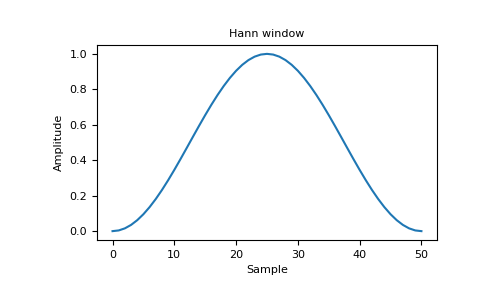
\includegraphics[width=0.8\textwidth, keepaspectratio]{images/hann_window.png}
  \caption{Von Hann Fensterfunktion \autocite{noauthor_numpyhanning_nodate}}
  \label{fig:vonHannFenster}
\end{figure}
Um die bei der Unterteilung des Audiosignals entstandenen Diskontinuitäten aufzulösen, wird eine Fensterfunktion auf die einzelnen Blöcke angewendet.
Abbildung~\ref{fig:vonHannFenster} zeigt die von Hann Fensterfunktion, welche neben dem Hamming Fenster zu den typischen Fensterfunktionen in der Audiosignalverarbeitung zählt.
Durch den Nulldurchgang am Anfang und Ende der Fensterfunktion werden die Amplituden des Blocksignals nach Anwenden der Funktion an den Grenzen auf Null gezogen, wodurch sich ein kontinuierlicher, periodischer Signalverlauf ergibt \autocite[vgl.][S. 462]{richter_signal_2022}.

Wird der Schritt des Windowing nicht durchgeführt, führt dies zu einem Phänomen namens spectral leakage.
Bei der Transformation des Signals von dem Zeitbereich in den Frequenzbereich resultiert der Amplitudensprung an den Blockenden in der Registrierung einer Vielzahl von Frequenzen.
Wie der Name bereits beschreibt, wird aus einer eindeutigen Frequenz, ein Spektrum aus Frequenzen, die nicht Teil des Signals sind \autocite[vgl.][S. 1296]{wu_new_2012}.

%%%% paste from t3000

\subsubsection{Fourier Analyse}
Die Grundlage für die Fourier Analyse stellt die von Jean-Baptiste Joseph Fourier entwickelte Fourier Reihe dar.
In diesem Unterkapitel wird dabei zunächst die Fourier Reihe vorgestellt und anschließend die in dieser Arbeit verwendete \ac{FFT} daraus schrittweise abgeleitet.

\paragraph{Fourier-Reihe}

% Reihenentwicklung einer periodischen Funktion in Funktionsreihe aus Sinus- und Cosinusfunktionen

Die Fourier-Reihe ist ein Verfahren, mit dem eine periodische Funktion in eine unendliche Summe von Sinus- und Cosinusfunktionen zerlegt werden kann.
Wenn ein Signal $s(t)$ folgende Eigenschaften aufweist:

\begin{itemize}
    \item $s(t)$ ist periodisch mit der Periode $T$ (d.h. $s(t+T) = s(t)$)
    \item $s(t)$ ist stetig mit endlich vielen Sprungstellen im Intervall $[0,T]$
    \item $\int_{0}^{\infty} |s(t)| dt < \infty$
\end{itemize}

dann kann $s(t)$ in

\begin{equation}
s(t) = \frac{a_0}{2} + \sum_{n=1}^{\infty} a_n \cdot cos(n\omega_0t) + \sum_{n=1}^{\infty} b_n \cdot sin(n\omega_0t)
\end{equation}

zerlegt werden, wobei

\begin{equation}
a_0 = \frac{2}{T} \int_{0}^{T} s(t) dt
\end{equation}

\begin{equation}
a_n = \frac{2}{T} \int_{0}^{T} s(t) \cdot cos(n\omega_0t) dt
\end{equation}

\begin{equation}
b_n = \frac{2}{T} \int_{0}^{T} s(t) \cdot sin(n\omega_0t) dt
\end{equation}

\begin{equation}
\omega_0 = \frac{2\pi}{T}
\end{equation}

sind \autocite[vgl.][S. 19f]{ries_fourier-reihe_2018}.

Die Fourier-Koeffizienten $a_n$ und $b_n$ sagen also aus, wie stark einzelne Frequenzen in $s(t)$ vorkommen.
Diese Frequenzanteile sind als Output der Fourier-Reihe zu verstehen und können als Merkmale für periodische Signale verwendet werden.
$a_0$ ist der Mittelwert der Funktion $s(t)$.

\paragraph{Kontinuierliche Fourier-Transformation}

% Aperiodische Signale werden in kontinuierliches Spektrum zerlegt

Anders als bei der Fourier Reihe, können mit der verallgemeinerten kontinuierlichen Fourier-Transformation auch aperiodische Signale zerlegt werden, die folgende Eigenschaften aufweisen:

\begin{itemize}
    \item $s(t)$ ist stückweise stetig
    \item $\int_{-\infty}^{\infty} |s(t)| dt < \infty$
\end{itemize}

Die Fourier-Transformation liefert eine Transformierte Funktion $\underline{S}(f)$, die als Spektrum des Signals $s(t)$ bezeichnet wird.
Es wird also die Dimension Zeit $t$ in die Dimension Frequenz $f$ transformiert.
Die Formel für die Fourier-Transformation lautet:

\begin{equation}
    \underline{S}(f) = \int_{-\infty}^{\infty} s(t) \cdot e^{-j2\pi ft} dt
\end{equation}

Wie bereits an der Formel zu erkennen ist, ist das Ergebnis der Fourier-Transformation eine komplexe Funktion mit einem Realteil $\Re(\underline{S}(f))$ und einem Imaginärteil $\Im(\underline{S}(f))$.

Da bei der Weiterverarbeitung in der Regel nur der Normalteil des Spektrums benötigt wird, wird die Fourier-Transformation in der Praxis meistens in der Form

\begin{equation}
    \Re(\underline{S}(f)) = \int_{-\infty}^{\infty} s(t) \cdot cos(2\pi ft) dt
\end{equation}

durchgeführt \autocite[vgl.][S. 350f]{picard_fourier-analyse_1996}.

\paragraph{Diskrete Fourier-Transformation}

% Diskrete Signale werden in diskretes Spektrum zerlegt
Bei den bisherigen Analyseverfahren, wurden immer kontinuierliche Signale betrachtet.
Das heißt, dass für jeden Zeitpunkt $t$ ein Wert $s(t)$ existiert.

Bei der \ac{DFT} können diskrete Signale verarbeitet werden, die aus einer Folge von $N$ Werten ($s_0, s_1, \dots, s_{N-1}$) bestehen, weshalb diese Methode besonders interessant für elektronisch aufgezeichnete Signale ist.

Da keine kontinuierliche Funktion vorliegt, besteht keine Möglichkeit mehr, ein Integral zu bilden, weshalb die Formel mit einer Summe aufgestellt ist:

\begin{equation}
    S_k = \frac{1}{N} \sum_{n=0}^{N-1} s_n \cdot e^{-j2\pi \frac{kn}{N}}
\end{equation}

Der Output der \ac{DFT} ist wieder eine komplexe Wertereihe, deren Realteil $\Re(S_k)$ und Imaginärteil $\Im(S_k)$ die Amplitude und Phase der $k$-ten Frequenzkomponente des Signals $s_n$ beschreiben.
Der Realteil lässt sich durch die Umformung der Formel in die Form

\begin{equation}
    \Re(S_k) = \frac{2}{N} \sum_{n=0}^{N-1} s_n \cdot cos(2\pi \frac{kn}{N})
\end{equation}

berechnen \autocite[vgl.][S. 567ff]{smith_scientist_1997}.

Um auf die jeweiligen Frequenzanteile des Signals zu schließen, können die Output-Bins $S_k$ mit folgender Formel in die Frequenzen $f_k$ umgerechnet werden:
% TODO: Bins erklären

\begin{equation}
    f_k = \frac{k}{N} \cdot f_s
\end{equation}

wobei $f_s$ die Abtastrate des Signals ist.

\paragraph{Fast Fourier Transformation}

Die \ac{DFT} würde sich nach der obigen Formel implementieren und für jedes Signal nutzen lassen.
Allerdings ist die Komplexität der \ac{DFT} mit $\mathcal{O}(N^2)$ sehr hoch, weshalb die \ac{FFT} entwickelt wurde, die den gleichen Output liefert, aber mit einer Komplexität von $\mathcal{O}(N log(N))$ \autocite[vgl.][S. 338]{beucher_signale_2011}.

Die \ac{FFT} ist somit eine für Computer optimierte Implementierung der \ac{DFT}.
Eine genaue Erklärung, warum \ac{FFT} signifikant weniger Berechnungen benötigt, würde für diese Seminararbeit zu sehr ins Detail gehen.
Einfach gesagt, nutzt der Algorithmus die Eigenschaft von Sinus- und Cosinus-Wellen, dass Wellen mehrfacher Frequenz an bestimmten Stellen dieselben Werte annehmen und so nur einmal berechnet werden müssen.

\begin{figure}
    \centering
    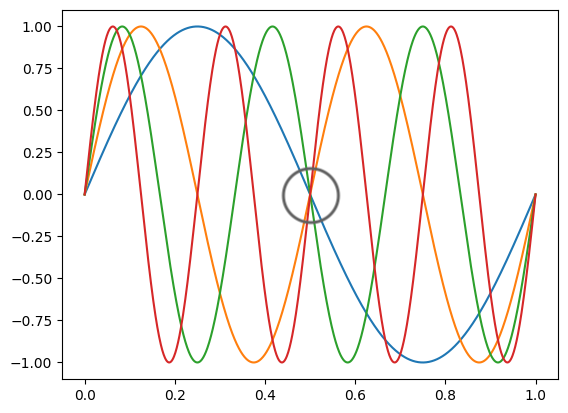
\includegraphics[width=0.5\textwidth]{images/fft-advantage.png}
    \caption{Sinuswellen mit 1hz, 2hz, 3hz, 4hz überlagern sich bei $t=0,5$}{Quelle: Eigene Darstellung}
    \label{fig:fft-advantage}
\end{figure}\noindent

Durch diese Eigenschaft und das rekursive Aufteilen des Signals in gerade und ungerade Datenpunkte spart der Algorithmus sehr viele Berechnungen ein \autocite[vgl.][S. 643]{oppenheim_discrete-time_1999}.

\subsubsection{Mel Frequency Cepstral Coefficients}
Die \ac{DFT} ermöglicht es bereits wesentliche Merkmale wie die Stimmlage und -farbe einer aufgezeichneten Stimme zu bestimmen.
Um die gewonnenen Merkmale der Fourier Analyse zu verbessern, werden weitere Berechnungsschritte durchgeführt, sodass die Merkmale in \ac{MFCC} umgewandelt werden.

Der Vorteil von Merkmalen wie \ac{MFCC} ist zunächst, dass Audio-Signale mit verschiedenen Längen und Abtastraten besser miteinander verglichen werden können.
Das liegt daran, dass bei einer Analyse der \ac{MFCC} eine fest definierbare Anzahl an Koeffizienten generiert werden.
Die Anzahl hängt dabei, anders als bei einer Fouriertransformation, nicht von der Frame-Länge und Abtastrate ab.
Zudem sind die \acp{MFCC} mehr auf die menschliche Wahrnehmung von Tönen abgestimmt und robuster gegenüber Hintergrundrauschen.

Um die \ac{MFCC} zu berechnen sind die folgenden vier Schritte notwendig \autocite[vgl. ][S. 2]{logan_mel_2000}:

\begin{enumerate}
    \item \textbf{\ac{DFT}}\\Bestimmung der Frequenzkomponenten
    \item \textbf{Logarithmierung}\\Näher an menschlicher Wahrnehmung
    \item \textbf{Abbildung auf die Mel-Skala}\\Zusammenfassung von Frequenzen zu Mel-Bändern mithilfe von Dreiecksfiltern
    \item \textbf{Diskrete Kosinustransformation}\\Ähnlich zur inversen Fourier-Transformation
\end{enumerate}

Durch die Abbildung der ermittelten Frequenzen auf die Mel-Skala orientiert sich das Verfahren somit an der menschlichen Stimmwahrnehmung, welche bereits im vorangehenden Kapitel erläutert wurde.

\subsubsection{Linear Predicitve Coding}
Die Grundlage von \ac{LPC} bildet das \ac{AR} Modell.
Die \ac{AR} basiert auf dem Konzept der multiplen Regression und wird auf zeitlich veränderliche Prozesse angewandt.
Dabei wird eine Kriteriumsvariable unter Betrachtung von einer beliebigen Anzahl an Prädiktorvariablen vorhergesagt \autocite[vgl.][S. 37-38]{canela_multiple_2019}.
Im speziellen Fall der \ac{AR} handelt es sich bei den Prädiktorvariablen um vorhergehende Werte des Prozesses.
Ein \ac{AR} Modell sagt somit den Wert zu einem Zeitpunkt $n$, basierend auf $p$ Vorgängerwerten des Prozesses voraus.
Es gilt somit der in Formel~\ref{eq:autoregression} dargestellte Zusammenhang, wobei $\hat{s}_n$ den vorausgesagten Wert, $s_{n-k}$ die vorhergehenden Werte, $a_{k}$ die Regressionsgewichte und $p$ die Anzahl an verwendeten Vorgängerwerten darstellt \autocite[][S. 1304]{atal_effectiveness_1974}.
\begin{equation}
  \hat{s}_{n} = \sum_{k=1}^{p} s_{n-k}a_{k}
  \label{eq:autoregression}
\end{equation}

Zur Bestimmung der Regressionsgewichte wurden verschiedene rekursive Verfahren entwickelt.
Neben der Yule-Walker Methode stellt der Burg Algorithmus eine beliebte Alternative dar, welcher in \citeauthor[][S. 443]{marple_new_1980} beschrieben ist.
% TODO: Formeln evtl. mit in die Arbeit ziehen
% Evtl: Formeln des Burg Algorithmus auflisten und erklären
% Evtl: Was hat Yule-Walker und Levinson damit zu tun?

Bei dem Verfahren \ac{LPC} wird der Ansatz verfolgt, Rückschlüsse von dem akustischen Signal auf die Stimmerzeugung zu ziehen.
Dazu wird ein \ac{AR}-Filter verwendet, um ein vereinfachtes Modell des menschlichen Stimmtrakts zu erstellen.
Die Regressionsgewichte $a_k$ entsprechen dabei den \ac{LPC}-Koeffizienten.
% TODO: Genauer erklären warum die Gewichte eine Rolle spielen -> Stimmerzeugung mit Grundrauschen + Koeffizienten als Filter

Das durch die \ac{LPC}-Koeffizienten erstellte Modell erfasst die Resonanzeigenschaften des Signals, wodurch Rückschlüsse auf die Formanten geschlossen werden können.
Da die Struktur der Formanten sprecherspezifisch ist, kann der Sprecher somit über die \ac{LPC}-Koeffizienten identifiziert werden \autocite[vgl.][S. 117]{sidorov_text-independent_2010}.

Zur Berechnung der \ac{LPC}-Koeffizienten wird zunächst die selbe Annahme wie in Kapitel~\ref{sec:Framing} getroffen, dass sich die Form des Vokaltrakts und das in den Stimmritzen erzeugte Signal über den betrachteten Zeitraum nicht verändert \autocite[vgl.][S. 1304]{atal_effectiveness_1974}.
Somit lassen sich die Koeffizienten des \ac{AR}-Filters mittels des Burg-Algorithmus berechnen.

\subsection{Künstliche Intelligenz}
\ac{KI} hat in den letzten Jahren stark an Aufmerksamkeit gewonnen und gilt als eine der wichtigsten Technologien des 21. Jahrhunderts.
Spätestens seit der Veröffentlichung und dem Erfolg durch den Chatbot ChatGPT am 30. November 2022 sind die Möglichkeiten von \ac{KI} den meisten Menschen bekannt. 
ChatGPT hat innerhalb von fünf Tagen die Schwelle von einer Million Nutzer erreicht. 
Spotify oder Facebook zum Vergleich haben hierfür 5 beziehungsweise 10 Monate benötigt \autocite[vgl. ][]{janson_infografik_2023}.

Die Statistik die im Jahr 2022 von der International Data Corperation erstellt wurde prognostiziert für die Anwendungsfelder Hardware, Software und IT-Services im Jahr 2024 einen weltweiten Umsatz von 554,3 Milliarden US-Dollar.
Dies entspricht einer Steigerung von 171 Milliarden US-Dollar (44,6 \%) im Vergleich zum Jahr 2021 \autocite[vgl. ][]{idc_kunstliche_2022}.
Dies unterstreicht noch einmal die Relevanz von \ac{KI} im aktuellen Zeitalter.
Doch was ist \ac{KI} und wie ist Sie für diese Arbeit von Relevanz, diese Fragen werden im Folgenden beantwortet.

Die Idee einer \acl{KI} ist bereits seit Mitte des 20. Jahrhunderts existent. 1955 definierte John McCarthy, einer der Pioniere der \ac{KI}, als erster den Begriff der \acl{KI} wie folgt:
\begin{quote}
  \gqq{Ziel der KI ist es, Maschinen zu entwickeln, die sich verhalten, als verfügten sie über Intelligenz.}
  \autocite[][S. 1]{ertel_grundkurs_2016}
\end{quote}\noindent
Aus heutiger Sicht ist diese Definition nicht mehr ausreichend.
Eine weit verbreitete Definition stammt von Elaine Rich welche sagt, dass sich \ac{KI} mit der Entwicklung von Computeralgorithmen befasse, für Probleme, die Menschen im Moment noch besser lösen können \autocite[vgl. ][]{rich_artificial_1983}.
%Themenfelder KI

Aufgrund der Entwicklung seit Mitte des 20. Jahrhunderts gliedert sich das Thema \ac{KI} in viele Teilgebiete.
% letztes Jahrzent vorallem Fortschritte im Bereich ML / grundsätzlich Lernen, welches relevant ist für Arbeit
Die verschiedenen Teilgebiete sind in der Abbildung \ref{fig:KI-Teilgebiete} dargestellt.
\begin{figure}[H]
    \centering
    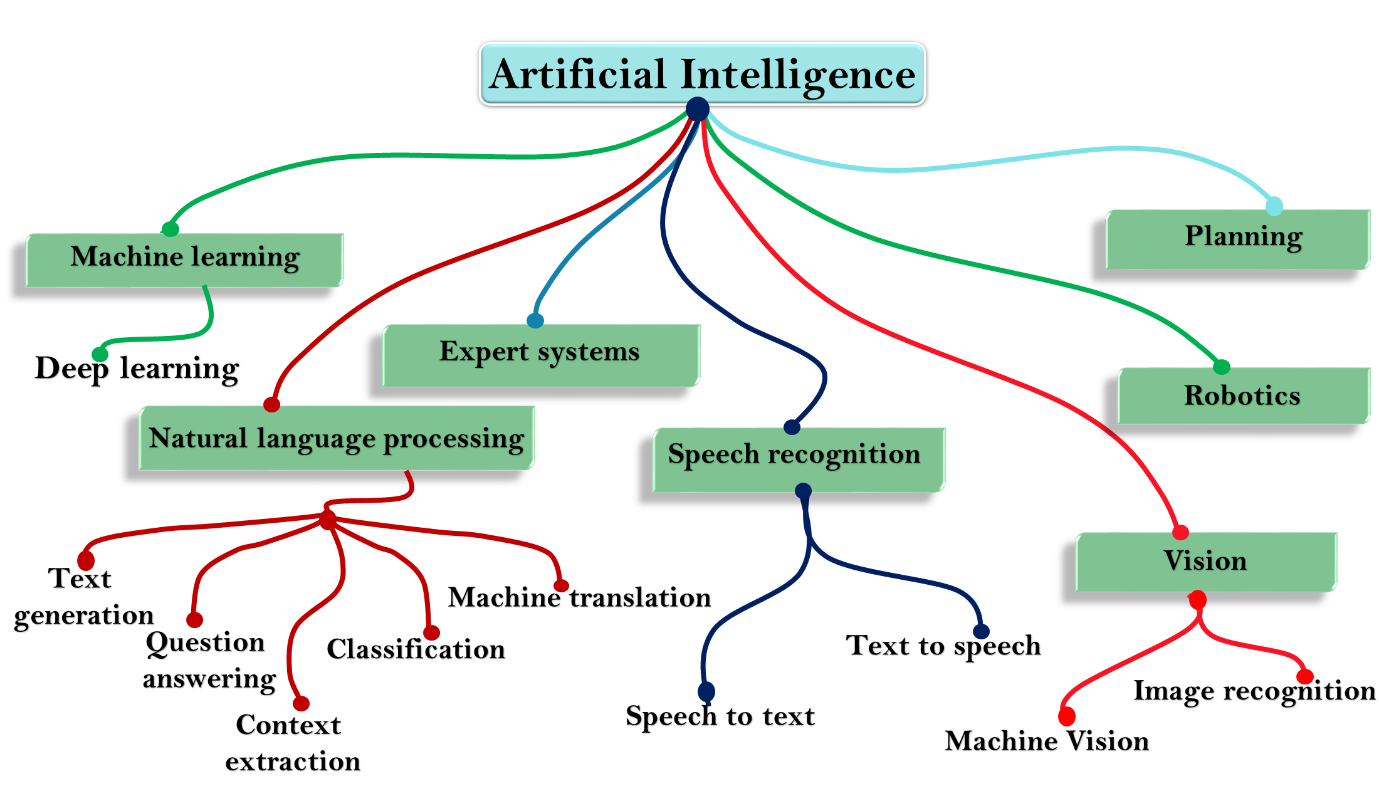
\includegraphics[width=0.9\textwidth]{images/KI_teilgebiete.png}
    \customcaption{Teilgebiete Künstliche Intelligenz}{\autocite[vgl.][]{noauthor_subsets_nodate}}
    \label{fig:KI-Teilgebiete}
\end{figure}\noindent
Insbesondere das Thema \ac{ML} hat in den letzten zehn Jahren viel Beachtung gefunden. 
\ac{ML} spielt für diese Studienarbeit eine entscheidende Rolle und wird deshalb im folgenden genauer betrachtet.
\newline
\ac{ML} ist nicht neu, bereits in den 1950er Jahren wurden von Arthur Lee Samuels die ersten \ac{ML} Programme entwickelt \autocite[vgl.][S. 5]{judith_hurwitz_machine_2018}.
Der Aufschwung von \ac{ML} im letzten Jahrzehnt ist auf steigende und bezahlbare Rechenleistung bzw. Speichergrößen zurückzuführen.
\ac{ML} beschreibt den Prozess bei dem Computeralgorithmen trainiert werden, um ihre Leistung bei einer bestimmten Aufgabe zu verbessern ohne dass dies explizit programmiert werden muss.
Hierzu werden dem Computer Daten bereitgestellt aus welchen er lernt.
Der Computer kann anschließend aus den Daten gewonnenen Erkenntnisse nutzen, um Vorhersagen für neue Daten zu treffen \autocite[vgl.][S. 4]{judith_hurwitz_machine_2018}.
% Beispielsweise wird dem Computer eine Liste mit Häusern, deren Eigenschaften (z.B. Anzahl Zimmer, Wohnfläche, Alter und Standort) und einem Verkaufspreis zu Verfügung gestellt.
% Mit \ac{ML} wird ein Modell trainiert, das die Auswirkungen der Eigenschaften auf den Verkaufspreis analysiert.
% Dieses Modell kann verwendet werden, um den Verkaufspreis von anderen Häusern vorherzusagen.
Die Vorhersagen stimmen nicht immer zu 100 \%, die Vorhersagegenauigkeit hängt von verschiedenen Faktoren ab, welche je nach Anwendungsfall variieren.
\newline
\ac{ML} lässt sich in die drei Kategorien überwachtes Lernen, unüberwachtes Lernen und verstärkendes Lernen gliedern.
Beim überwachten Lernen besteht der Trainingsdatensatz aus Eingabewerten und gewünschten Ausgabewerten.
Der Algorithmus generiert eine Abbildungsfunktion, die die Eingabewerte auf die Ausgabewerte abbildet.
Der Computer wird sozusagen unterrichtet, Vorhersagen für zukünftige Daten auf Grundlage von Bestandsdaten zu erstellen \autocite[vgl][S. 11]{thakkar_beginning_2019}.
Im Gegensatz dazu besteht der Trainingsdatensatz beim unüberwachten Lernen nur aus unmarkierten Eingabewerten.
Das Ziel von unüberwachtem Lernen besteht darin Muster oder Strukturen zu erkennen.
Der Computer unterrichtet sich sozusagen selbst \autocites[vgl.][S. 11-12]{thakkar_beginning_2019}[vgl.][S. 6]{etaati_machine_2019}.
Verstärkendes Lernen ist ein verhaltensbasiertes Lernmodell.
Hierzu interagiert der Lernalgorithmus mit der Umgebung und erhält Belohnungen, wenn er die gewünschten Ergebnisse erzielt. 
Der Computer erlernt so das ideale Verhalten innerhalb der Umgebung \autocite[vgl][S. 12]{thakkar_beginning_2019}.

\subsection{Neuronale Netze}\label{sec:neuronaleNetze}
In engem Zusammenhang zu \acl{ML} stehen die sogenannten \aclp{NN}.
Ein \ac{NN} ist ein maschinelles Modell, das auf dem Vorbild der Abläufe im Gehirn von Mensch und Tier basiert.
Durch geeignete mathematische Operationen wird versucht die Art und Weise abzubilden wie das menschliche Gehirn Probleme angeht beziehungsweise Zusammenhänge aus beobachteten Daten erkennt \autocites[vgl.][S. 604]{backhaus_multivariate_2016}[vgl.][S. 31]{judith_hurwitz_machine_2018}.
Aus den vorhin genannten Lernalgorithmen (überwachtes, unüberwachtes, und verstärkendes Lernen) ergibt sich als Ergebnis ein neuronales Netz, welches das erlernte Wissen in seiner Struktur speichert \autocite[vgl.][S. 427]{guresen_definition_2011}.

%Aufbau von neuronalen Netzen
Ein neuronales Netz ist prinzipiell in Schichten aufgebaut.
In jedem neuronalen Netz gibt es eine Eingabe- und Ausgabeschicht.
Zwischen der Eingabe- und Ausgabeschicht liegen mehrere versteckte Schichten (hidden layers).
Jede Schicht besteht aus mehreren Neuronen (Knoten), welche über gewichtete Kanten miteinander verbunden sind \autocite[vgl.][S. 26]{sonnet_neuronale_2022}.
Die Informationen werden durch die Neuronen in der Eingabeschicht aufgenommen und durch die Neuronen in der Ausgabeschicht ausgegeben.
Die Neuronen in der versteckten Schicht verarbeiten die Informationen.
Ein grundsätzlicher Aufbau eines neuronalen Netzes ist in Abb. \ref{fig:StructureNN} dargestellt.
\begin{figure}[H]
    \centering
    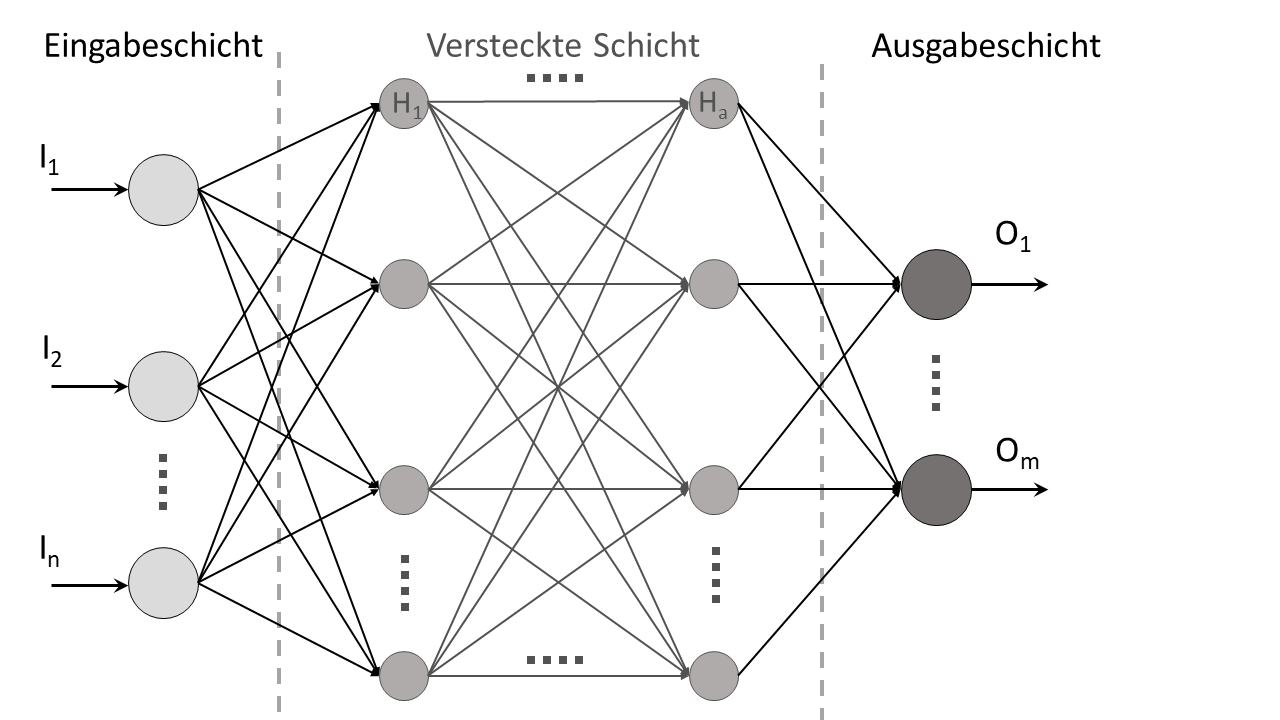
\includegraphics[width=0.9\textwidth]{images/structure_NN.png}
    \customcaption{Grundsätzlicher Aufbau eines neuronalen Netzes}{\autocite[][]{daniel_john_neuronales_2022}}
    \label{fig:StructureNN}
\end{figure}\noindent
Ein Neuron ermittelt seine Aktivierung aufgrund der Eingaben der vorherigen Neuronen und gibt daraus aufbauend einen Wert aus.
Dieser Wert kann durch die Gewichte auf den Kanten beeinflusst werden.
Von der Aktivierung ist abhängig, ob das Neuron feuert, sprich seinen errechneten Wert weitergibt.
Dies gibt Aufschluss über die Relevanz die vorangegangenen Werte.
% //TODO Quelle dazu suchen sonst \autocite[vgl.][S. 27]{sonnet_neuronale_2022}. beschreibt aber nut Aktivierung nicht was dies bedeutet
Somit können durch die Gewichte der Kanten und den Wert der Neuronen Informationen abgebildet werden.
\autocite[vgl.][S. 27]{sonnet_neuronale_2022}

Für das Training von neuronalen Netzen werden viele klassifizierte Daten benötigt, welche als Ausgangspunkt dienen.
Das Training läuft iterativ in Schleifen, in sogenannte Epochen ab.
Nach jedem Durchlauf werden mithilfe des Feedbacks der Ausgabeschicht die Gewichte der Kanten und der Wert der Neuronen angepasst.
Zu Beginn werden die Kanten-Gewichte und der Wert eines Neurons zufällig gesetzt.
Dies wirkt sich auf das Ergebnis des gesamten Trainingsprozesses aus, da die zufällig gesetzten Werte so ungünstig sein können, dass das Netz während des Durchlaufs die Gewichte nicht ausreichend anpassen kann.
Nach Abschluss des Trainings kann das Netz bewertet werden.
Hierbei werden abhängig von der gewählten Technologie unterschiedlich Parameter ausgegeben.
Grundsätzlich kann ein Netz immer beurteilt werden indem bereits klassifizierte Daten durch das Netz klassifiziert werden und die Ergebnisse anschließend mit dem tatsächlichen Ergebnis verglichen werden.
Im Regelfall werden hierbei Daten verwendet, welche zwar aus dem gleichen Datensatz stammen, jedoch nicht für das Training genutzt wurden.
\autocite[vgl.][]{marcel_mikl_wie_2018}
% Arten von NN

\subsection{Gefahrenanalyse (Attack Trees)}
Eine Möglichkeit der Beurteilung von sicherheitskritischen Systemen stellt die Gefahrenanalyse dar.
Dabei wird durch verschiedene Herangehensweisen versucht, möglichst viele potentielle Gefahren und Angriffsstellen des Systems zu ermitteln und anschließend zu bewerten.
Als Resultat ergibt sich eine klare Einschätzung der Gefahrensituation, wodurch eine Aussage über die Sicherheit des entwickelten Systems getroffen werden kann.

Eine Vorgehensweise stellen dabei die sogenannten Attack Trees dar.
Sie ermöglichen es in erster Linie, Gefahren strukturiert zu verwalten und übersichtlich darzustellen.
Mittels einer Baumstruktur werden dabei Gefahren Schicht für Schicht in ihre Komponenten zerlegt.
Dabei können Komponenten eines Elements entweder durch eine \gqq{oder} oder eine \gqq{und} Verknüpfung verbunden werden.
Somit kann definiert werden ob für das Eintreten einer Gefahr lediglich eine Komponente oder eine Kombination von Komponenten eintreffen muss.

Um festzustellen ob bereits alle Gefahren gefunden wurden, muss für jedes Element überprüft werden, ob es zusätzliche Wege gibt diese Gefahr zu erreichen.
Dabei können neben der eigenen Erfahrung auch zusätzliche Quellen wie das Internet oder bereits existierende Attack Trees herangezogen werden.
Wichtig ist dabei, dass auch von dem System bereits abgedeckte Gefahren mit aufgelistet und als solche markiert werden, sodass für den Betrachter ersichtlich wird, dass die Gefahr berücksichtigt wird \autocite[vgl.][S. 88-94]{shostack_threat_2014}.

Nachdem der Attack Tree aufgestellt ist, können verschiedene Auswertungen durchgeführt werden.
Dabei handelt es sich grundsätzlich um subjektive Einschätzungen.
Beispielhaft kann eine binäre Einteilung der Basisgefahren in \gqq{möglich} und \gqq{unmöglich} stattfinden.
Durch die Verknüpfungsregeln kann somit die Einteilung der Elternknoten ermittelt werden.

  \section{Stand der Technik}

\subsection{Feature Extraction}

Dieses Kapitel gibt 
  \section{Konzeption}\label{sec:Konzeption}

Das vorliegende Kapitel behandelt die Konzeption des Versuchssystems und des Demosystems.
Dazu erfolgt zuvor ein grobes Konzept für ein generisches Sprecherauthentifikationssystem und die Festlegung der Anforderungen an das Demo-System.

\subsection{Allgemeiner System-Aufbau}

Ein allgemeiner, generischer Aufbau für ein Sprecherauthentifikationssystem ist in Abbildung~\ref{fig:allg-generisch-aufbau} dargestellt.

Das Konzept wurde weitgehend eigens entwickelt, orientiert sich aber an den Ansätzen von Qi (Peter) Li \autocite[vgl. ][S. 7]{li_speaker_2012}.

\begin{figure}[H]
    \centering
    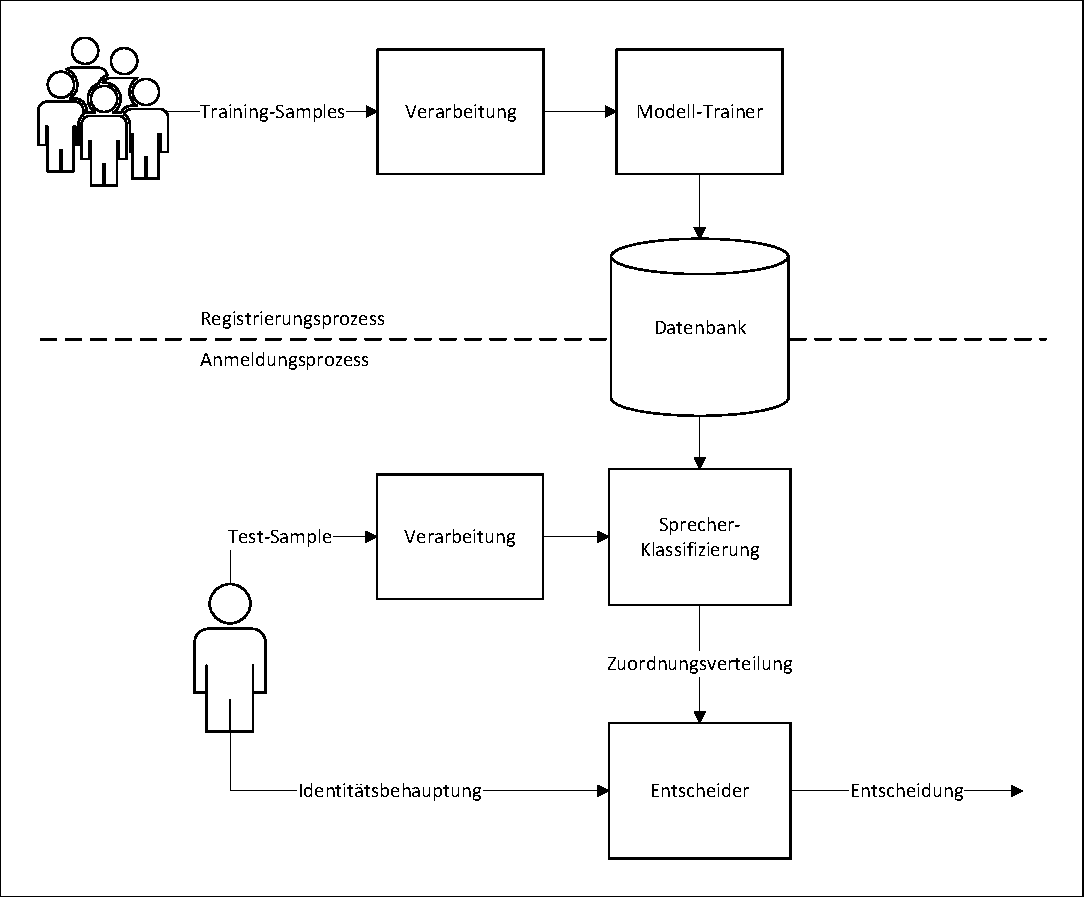
\includegraphics[width=\textwidth, keepaspectratio]{images/allg-generisch-aufbau.pdf}
    \caption{Informelles Komponentenkonzept für ein Sprecherauthentifikationssystem}
    \label{fig:allg-generisch-aufbau}
\end{figure}\noindent

Das System lässt sich in zwei Prozesse aufteilen: dem Registierungs- oder Trainingsprozess und dem Anmeldungs- oder Testprozess.
Die verschiedenen Komponenten der beiden Prozesse werden im folgenden Abschnitt kurz erklärt.

Am Anfang des Trainingsprozesses steht die Benutzergruppe.
Diese beinhaltet alle Personen, die das System benutzen wollen, beziehungsweise sich authentifizieren möchten.
Die Benutzer geben Trainings-Samples in eine Verarbeitungs-Komponente, welche die Audio-Daten so aufbereitet, dass sie für ein Modell verwendet werden können.
Die Modell-Trainer-Komponente generiert dann über mathematische Methoden eine Art Datenbank (zum Beispiel in Form eines neuronalen Netzes).
Dies ist die Schnittstelle zum Anmeldungsprozess.
In diesem möchte sich ein einzelner Benutzer mit dem System authentifizieren.
Dazu wird zunächst ein Test-Sample über eine Verarbeitungs-Komponente in die Sprecher-Klassifizierungs-Komponente gegeben, welche unter Verwendung der Datenbank-Komponente eine Zuordnungsverteilung erstellt.
Außerdem gibt der Nutzer eine Identitätsbehauptung ab, welche zusammen mit der Zuordnungsverteilung von einer Entscheidungs-Komponente verarbeitet wird.
Hieraus resultiert eine Entscheidung, ob die Identitätsbehauptung akzeptiert wird oder nicht.

\textauthor{\vJB,}{\vLB}{}

\subsection{Festlegung der Systemanforderungen}\label{sec:anforderungen}

Die grundlegende praktische Anforderung an diese Studienarbeit ist es, ein Sprecherauthentifikationssystem zu entwickeln, welches über eine Webapplikation bedient werden kann.
Dazu müssen geeignete Stimmmerkmale zur Benutzerauthentifizierung evaluiert werden.
Da diese Anforderungsbeschreibung noch viel Spielraum über den Funktionsumfang dieses Systems lässt, werden in diesem Kapitel die Anforderungen an das System genauer spezifiziert.

\begin{itemize}
    \item Das System soll lediglich ein Demosystem darstellen, welches die Machbarkeit eines Sprecherauthentifikationssystem aufzeigt. Es soll nicht in einem produktiven Umfeld eingesetzt werden können.
    \item Das System soll eine text-unabhängige Authentifizierung implementieren, da der Fokus des Systems auf der Identifikation von Stimmmerkmalen zur Authentifizierung von Benutzern liegt und dies unabhängig vom gesprochenen Text erfolgen soll.
    \item Der Datensatz für das System ist zu Beginn festgelegt. Das heißt, es können sich nur 20 bereits bekannte Sprecher authentifizieren. Zudem können keine neuen Sprecher registriert werden, wodurch das Sprecherauthentifikationssystem keine dynamische Erweiterung um Sprecher bereitstellen muss.
    \item Das System soll eine Open-Set-Implementierung verwenden. Dadurch wird sichergestellt, dass ein Benutzer erst mit einer fest definierten Sicherheit authentifiziert wird.
    \item Zur Authentifizierung eines Sprechers wird ein 15-sekündiger Audio-Clip an das System übermittelt. Der Audio-Clip ist dem System bisher unbekannt, aber in gleichen Bedingungen aufgenommen, wie die Clips des Trainingsprozesses.
    \item Das Sprecherauthentifikationssystem sollte Teil des Back-Ends sein. Die Bedienung erfolgt über eine Webapplikation, die mit dem System über eine Schnittstelle kommuniziert.
    \item In der Web-Oberfläche des Demosystems soll der zu authentifizierende Sprecher (einer der 20) und ein Verifikations-Clip ausgewählt werden können. Es soll für jeden Sprecher mindestens 5 Clips zur Auswahl geben.
    \item So soll der Nutzer des Demosystems testen können, was passiert, wenn ein zu dem zu authentifizierenden Sprecher passender bzw. unpassender Verifikations-Clip ins System gegeben wird.
    \item Das System soll dem Nutzer dann Informationen über die Identifikations-Verteilung (zu welchem Sprecher passt der Clip zu welchem Prozentsatz) und den Authentifizierungs-Status (\gqq{erfolgreich}/\gqq{nicht erfolgreich}) als Rückmeldung darstellen.
\end{itemize}

\textauthor{\vJB,}{\vLB}{}

\subsection{Konzept Versuchssystem}\label{sec:KonzeptVersuchssystem}
Die Konzeption des Versuchssystems unterteilt sich in mehrere Unterkapitel.
Zunächst wird die allgemeine Systemidee vorgestellt.
Anschließend wird auf die in dieser Arbeit evaluierten Feature Kombinationen eingegangen.
Daraufhin werden die Anforderungen an den Datensatz konkretisiert, woraufhin anschließend noch einmal auf den allgemeinen Verarbeitungsprozess der Audiodateien eingegangen wird.
Abgeschlossen wird das Kapitel mit einer Beschreibung der Klassifikation und Evaluierung, sowie der spezifischen Softwarearchitektur des Versuchssystems.

\subsubsection{Systemidee}

Aus der Literaturrecherche in Kapitel \ref{stand_der_technik} gehen verschiedene Stimmmerkmale zur Benutzerauthentifizierung hervor.
Die Ergebnisse der dargestellten Untersuchungen unterscheiden sich darin, inwieweit die unterschiedlichen Stimmmerkmale die Stimme repräsentieren bzw. zuverlässig für eine korrekte Authentifizierung sind.

Da die Features \ac{LPC}, \ac{LPCC}, \ac{MFCC} und \ac{dMFCC} die grobe Schnittmenge der Untersuchungen darstellt, werden diese in einer eigens durchgeführten Versuchsreihe getestet und evaluiert.
Hierfür wird ein System entworfen, das die Merkmale aus einem Datenset extrahiert und verschiedene Kombinationen vergleicht.
Das Ziel dieses Systems ist, eine ideale Kombination aus Features herauszufinden.
Ein grober Ablaufplan des Systems ist in Abbildung~\ref{fig:PAP_DemoSystem} dargestellt.
\begin{figure}[H]
    \centering
    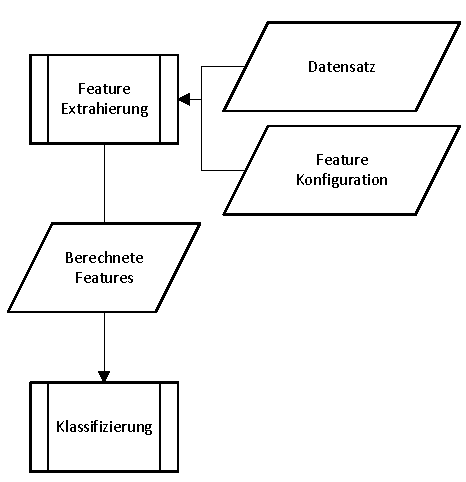
\includegraphics[width=0.6\textwidth, keepaspectratio]{images/PAP_Demosystem.pdf}
    \caption{Ablauf Versuchssystem}
    \label{fig:PAP_DemoSystem}
\end{figure}

% Dazu werden in einem ersten Schritt Konfigurationen definiert, welche die unterschiedlichen Zusammensetzungen der Features beschreibt.
% Anschließend werden alles diese Zusammensetzungen berechnet und durch neuronale Netze klassifiziert.
% Abschließend erfolgt eine Auswertung der verschiedenen Konfigurationen, um eine ideale Konfiguration von Features zu ermitteln

\subsubsection{Feature Kombinationen}\label{sec:FeatureKombination}

Um die Kombinationen zu generieren, werden zunächst die verschiedenen Möglichkeiten definiert und anschließend miteinander kombiniert, was zu über 500 verschiedenen Konfigurationen führt.
Hierzu werden zusätzlich zu den oben genannten Features auch die Anzahl und Länge der Frames definiert.
Für die Anzahl der Frames wurden 10000 und 15000 Frames definiert, für die Länge der Frames 400 und 600 Samples.
Diese Werte berechnen sich aus vorherigen Versuchen, der verwendeten Abtastrate und der gewünschten Trainingsclip-Länge.
Für die Features werden die Anzahl der Features pro Frame auf 13 und 20 festgelegt.
Der Wert 13 ist aus der Literatur abgeleitet \autocite[vgl.][S. 69]{valerio_velardo_mel-frequency_2020}.
Der Wert 20 ist selbstständig ergänzt, um einen Vergleich zu ermöglichen.
Da die Relevanz von \ac{dMFCC} am geringsten ist (s. Abb.~\ref{fig:vergleichFeatureExtraction}), wird hier auf den zweiten Wert verzichtet, um die Anzahl der Konfigurationen zu reduzieren.
Die vorhin genannten Werte sind übersichtlich in der nachfolgenden Tabelle dargestellt.
\begin{table}[H]
    \centering
    \begin{tabular}{l|l}
        \textbf{Bezeichner} & \textbf{Werte}   \\ \hline
        Anzahl der Frames   & 10000, 15000 \\ \hline
        Länge der Frames    & 400, 600     \\ \hline
        LPC                 & 13, 20       \\ \hline
        MFCC                & 13, 20       \\ \hline
        LPCC                & 13, 20       \\ \hline
        delta MFCC          & 13          
    \end{tabular}
    \caption{Übersicht Featurekombinationen}
\end{table}

% \begin{lstlisting}[language=JavaScript,numbers=none,caption=Konfigurationsmöglichkeiten,label=configs]
% Configs = {
%     "amount_of_frames": [10000, 15000],
%     "size_of_frame": [400, 600],
%     "LPC": {
%         "order": [13, 20],
%         "weight": [0, 1]
%     },
%     "MFCC": {
%         "order": [13, 20],
%         "weight": [0, 1]
%     },
%     "LPCC": {
%         "order": [13, 20],
%         "weight": [0, 1]
%     },
%     "delta_MFCC": {
%         "order": [13],
%         "weight": [0, 1]
%     }
% }
% \end{lstlisting}

% Die Werte für die Anzahl und Länge der Frames \codestyle{amount_of_frames} und \codestyle{size_of_frame} berechnen sich aus vorherigen Versuchen, der verwendeten Abtastrate und der gewünschten Trainingsclip-Länge.


% Bei den Features gibt der \codestyle{order} Parameter die Anzahl der Features pro Frame an.
% Der Wert 13 ist aus der Literatur abgeleitet. %TODO CITE
% Der Wert 20 ist selbstständig ergänzt, um einen Vergleich zu ermöglichen.
% Um die Anzahl der Konfigurationen zu reduzieren und da die Relevanz von \ac{dMFCC} am geringsten ist, wird hier auf den zweiten Wert verzichtet.
% Der \codestyle{weight} Parameter gibt lediglich an ob in dieser Konfiguration dieses Feature verwendet werden soll oder nicht.

\subsubsection{Datensatz} \label{sec:KonzeptDatensatz}
Um die unterschiedlichen Kombinationen an Features zu vergleichen, wird ein Datensatz benötigt, der mindestens 20 verschiedene Sprecher mit mindestens ca. 15 min unterschiedlichem Audio-Material enthält.
Die Audio-Clips müssen unter gleichen Bedingungen aufgenommen sein und in kompressionslosem WAV-Format vorliegen.
Der Datensatz wird aufgeteilt in Training- und Testdaten.

\subsubsection{Vorverarbeitung und Feature-Extraktion}

In der Feature Extraktion werden die Stimmmerkmale aus den Trainingsdaten extrahiert.
Hierzu müssen die Audiosignale zunächst vorverarbeitet werden (siehe Kapitel \ref{sec:preprocessing}).
In welcher Form die Merkmale extrahiert werden hängt dabei von der aktuellen Konfiguration ab.

Abbildung~\ref{fig:ablaufdiagramm-preprocessing-extraction} zeigt den Ablauf von diesem Teil des Versuchssystems mit Bezug auf die im Klassendiagramm dargestellten Klassen und Methoden (Abbildung~\ref{fig:klassendiagram-versuchssystem}).

\begin{figure}[H]
    \centering
    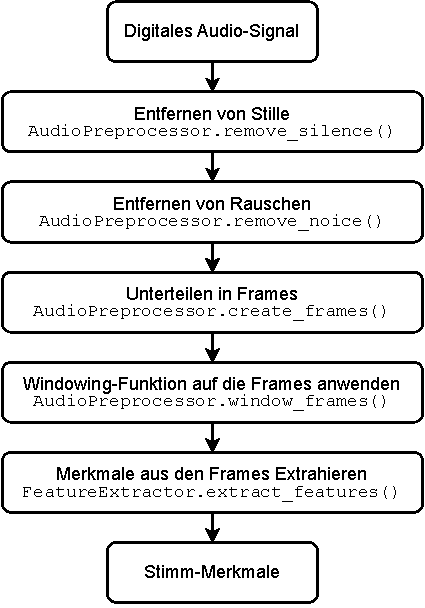
\includegraphics[width=0.4\textwidth, keepaspectratio]{images/ablaufdiagramm-preprocessing-extraction.pdf}
    \caption{Ablaufdiagramm Vorverarbeitung und Feature Extraktion}
    \label{fig:ablaufdiagramm-preprocessing-extraction}
\end{figure}\noindent

Näher wird dieser Ablauf in dem dazugehörigen Umsetzungs-Kapitel (\ref{section:umsetzung-versuch-vorverarbeitung}) beschrieben.

\subsubsection{Klassifikation und Evaluierung}\label{sec:KonzeptKlassifikation}

Die Literaturrecherche hat ergeben, dass sich neuronale Netze gut als Klassifikationsmodell eignen (siehe Kapitel \ref{stand_der_technik}). 
Deshalb werden bei der Klassifikation die berechneten Features aus dem Schritt zuvor genutzt, um neuronale Netze zu trainieren, sodass die Feature-Kombinationen bewertet werden können.
Hierbei muss das Netz mehrmals durchlaufen werden, da zu Beginn des Trainings die Gewichtung zufällig gesetzt wird (siehe Kapitel \ref{sec:neuronaleNetze}).
Anschließend werden die neuronalen Netze mit Testdaten getestet, die nicht in den Trainingsdaten enthalten sind.
Die Auswertung des neuronalen Netzes wird gespeichert und nach Berechnung aller Kombinationen ausgewertet.
Somit soll die beste Kombination gefunden und das damit trainierte neuronale Netz für das Demo-System verwendet werden.

\subsubsection{Software Architektur}
Um eine solide Grundlage für die Entwicklung zu schaffen, wird im Folgenden die Softwarearchitektur für das System entwickelt.
Hierzu wird zunächst basierend auf den vorangegangenen Definitionen ein Klassendiagramm erstellt.
In einem Folgeschritt wird der Ablauf in einem Sequenzdiagramm dargestellt. % optional
\newparagraph
Das Klassendiagramm ist in Abbildung~\ref{fig:klassendiagram-versuchssystem} dargestellt.
Es zeigt die Aufteilung des Systems in mehrere Komponenten (Klassen).
Die wichtigsten Klassen werden nachfolgend kurz beschrieben.
\begin{figure}[H]
    \centering
    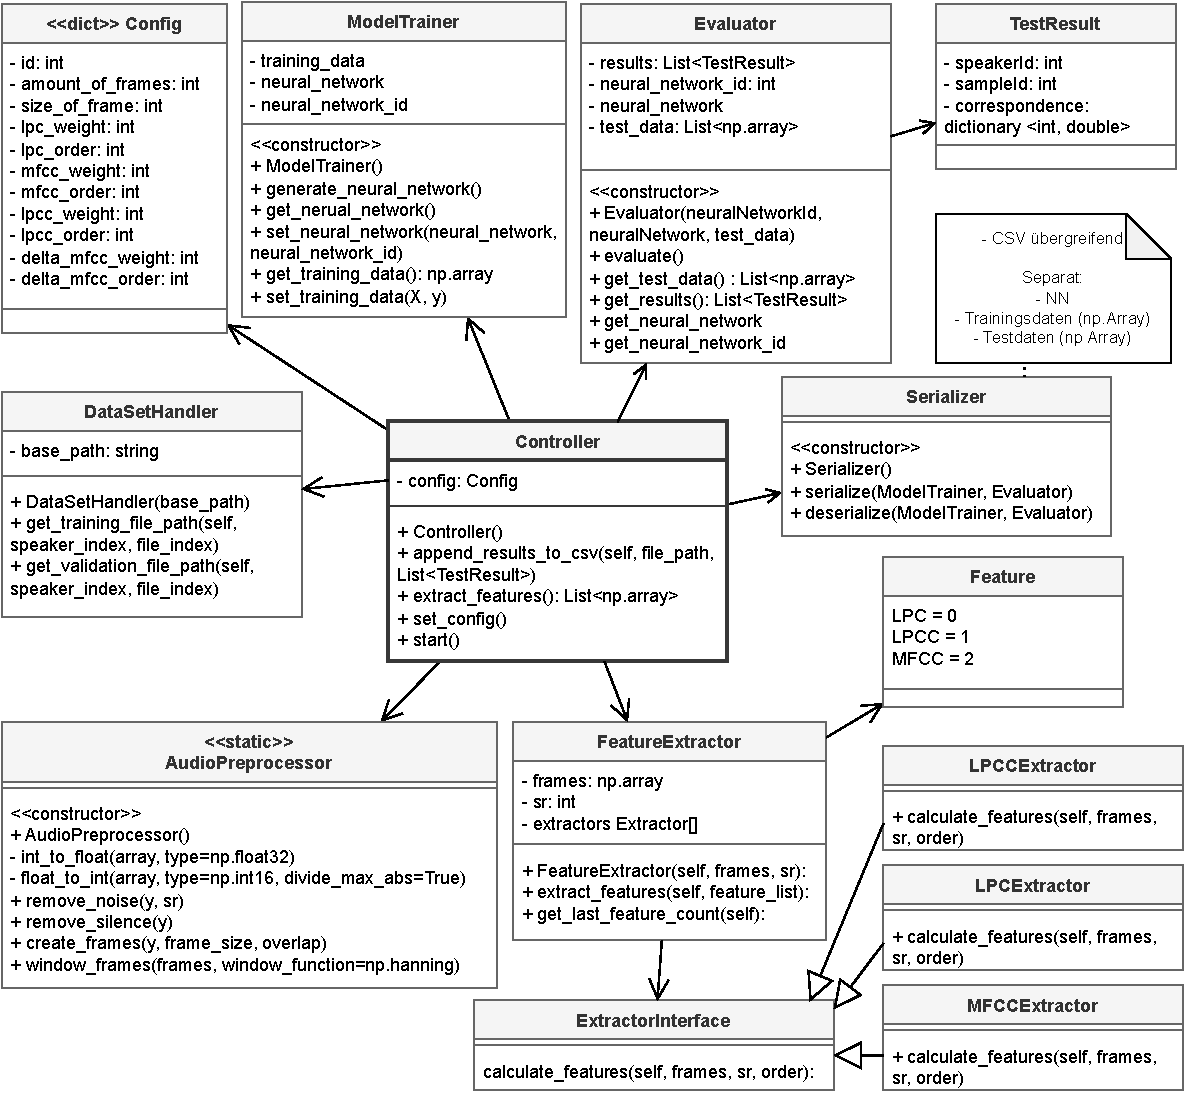
\includegraphics[width=\textwidth, keepaspectratio]{images/klassendiagram-versuchssystem.pdf}
    \caption{Klassendiagramm Versuchssystem}
    \label{fig:klassendiagram-versuchssystem}
\end{figure}\noindent


\noindent \textbf{Controller}\\
Der Controller stellt das zentrale Element dar, von hier werden alle Abläufe gesteuert.
\newline
\noindent \textbf{DatasetHandler}\\
Der DatasetHandler stellt die Verbindung zum Datenset dar und ermöglicht den Umgang mit den Dateien.
\newline
\noindent \textbf{AudioPreprocessor}\\
Der AudioPreprocessor dient im Allgemeinen zur Vorverarbeitung des Audiosignals.
\newline
\noindent \textbf{FeatureExtractor}\\
Mithilfe der FeatureExtractor-Klasse werden variabel die benötigten Audio-Merkmale aus den Audio-Clips generiert. Sie ruft die verschiedenen Implementierungen des ExtractorInterface auf.
\newline
\noindent \textbf{ModelTrainer}\\
Der ModelTrainer generiert und trainiert das neuronale Netz.
\newline
\noindent \textbf{Evaluator}\\
Mit dem Evaluator werden die neuronalen Netze auf ihre Genauigkeit geprüft.
\newline
\noindent \textbf{Serializer}\\
Die Serzializer-Klasse speichert die zu Laufzeit generierten Daten für weitere Untersuchungen.
\newparagraph

In Abb. \ref{fig:sequenzdiagramm-versuchssystem} ist das Sequenzdiagramm dargestellt, dies stellt den Durchlauf einer Konfiguration durch Objekte der verschiedenen Klassen dar.
\begin{figure}[H]
    \centering
    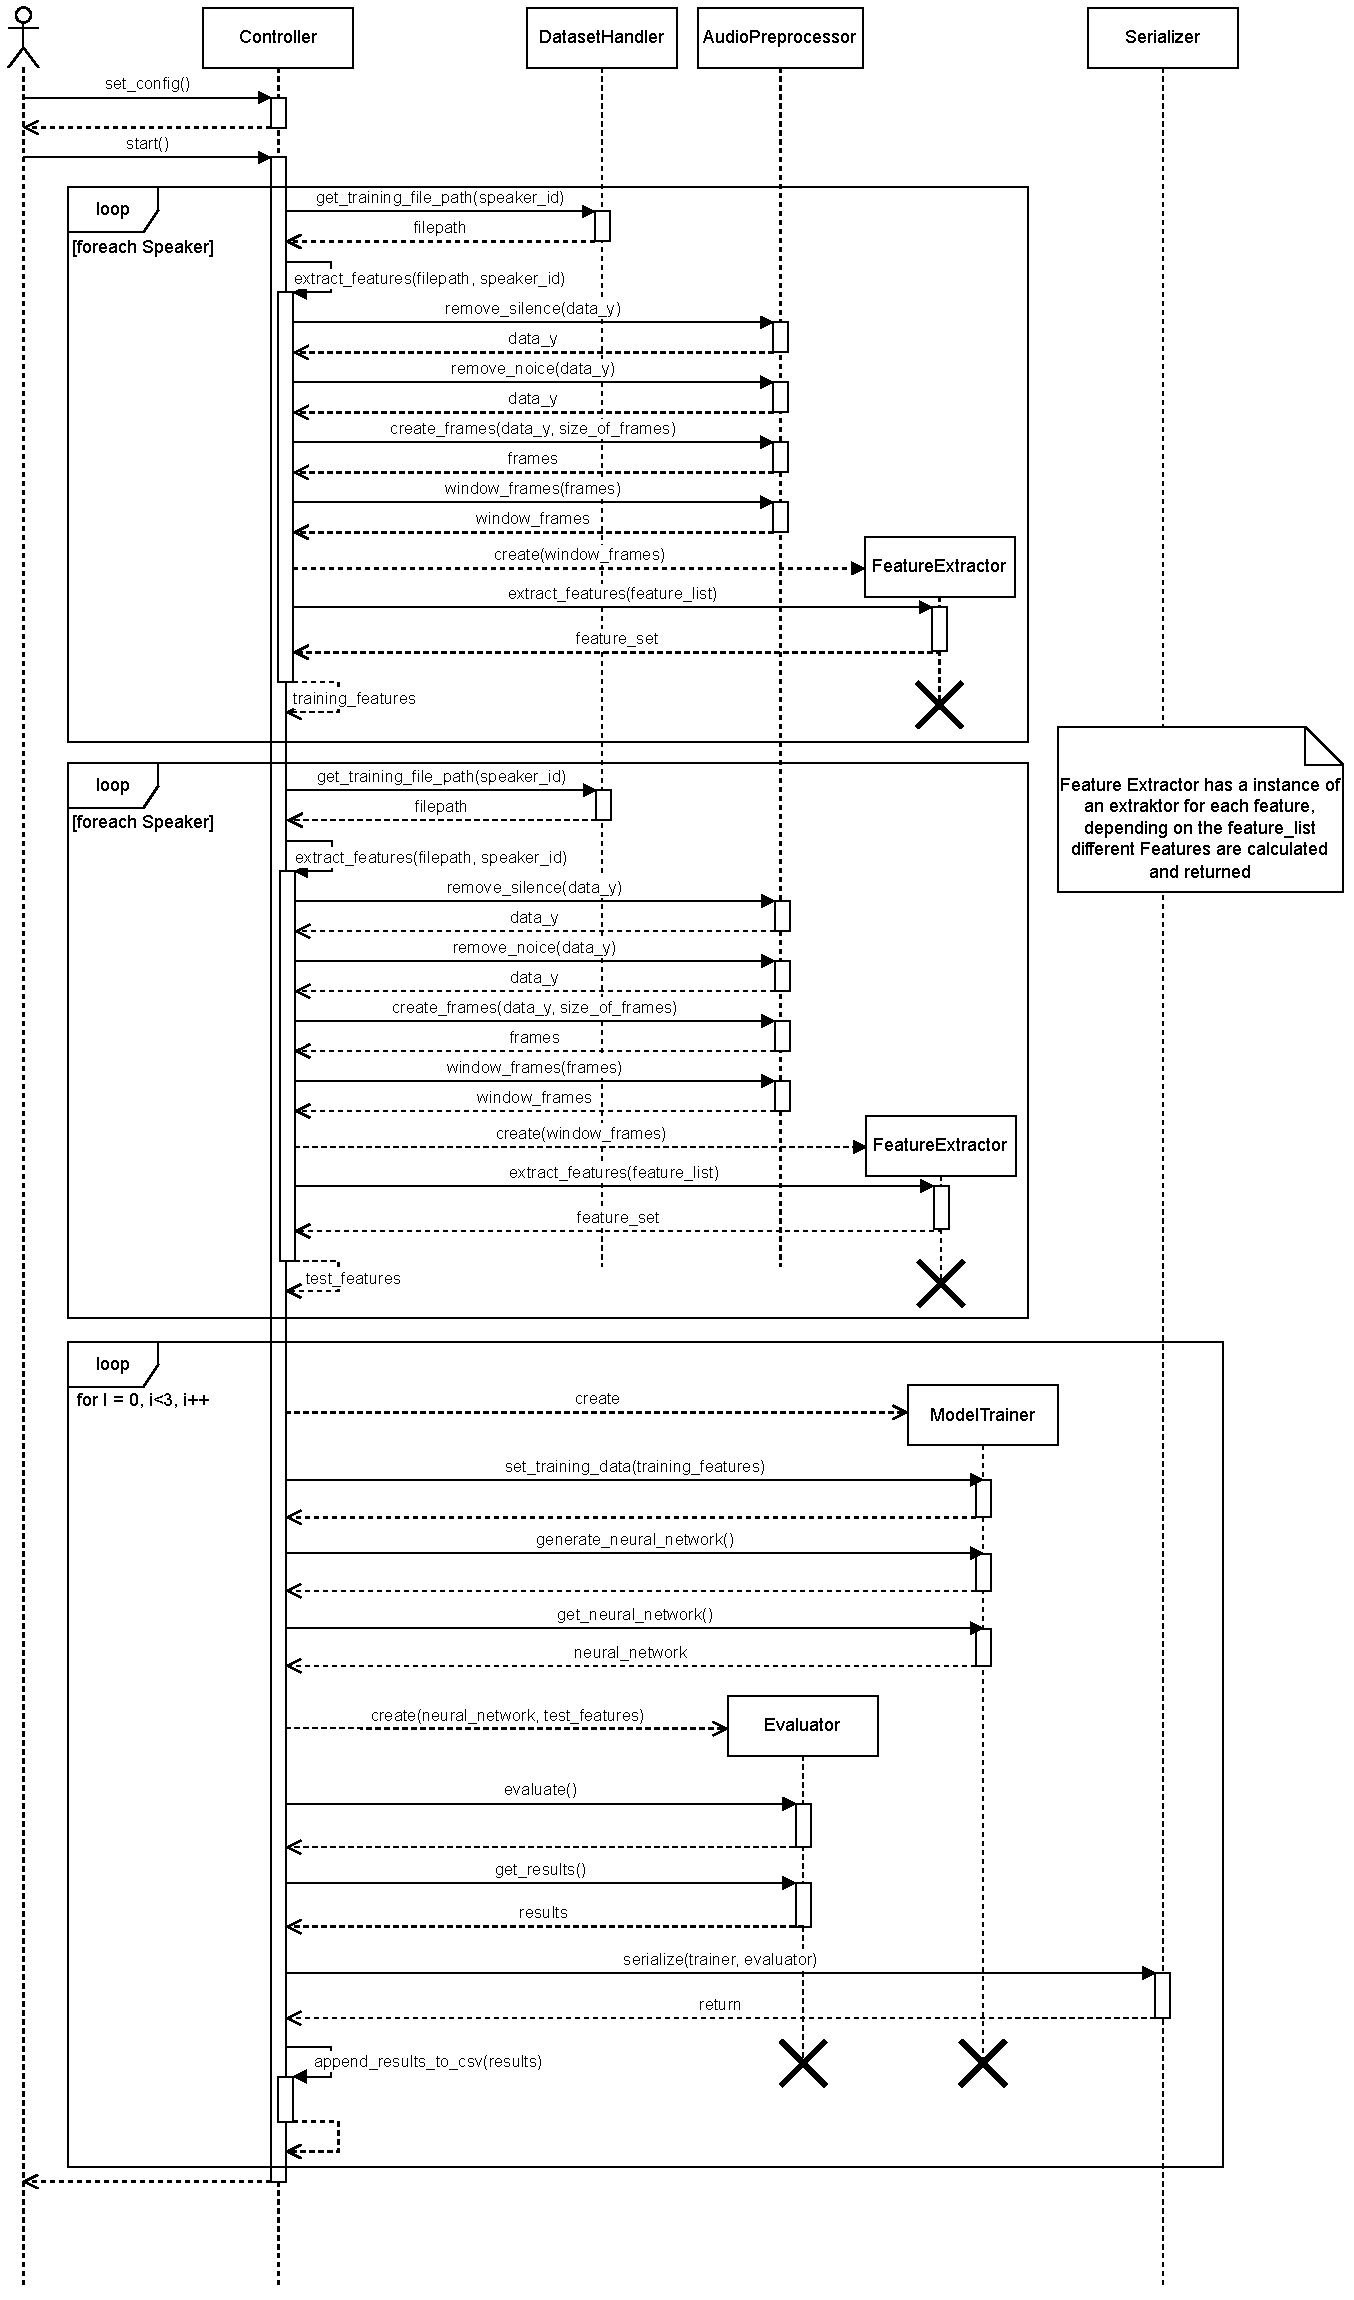
\includegraphics[width=0.82\textwidth, keepaspectratio]{images/versuchssytem_sequenzdiagramm.pdf}
    \caption{Sequenzdiagramm Versuchssystem}
    \label{fig:sequenzdiagramm-versuchssystem}
\end{figure}\noindent

% Beschreibung der Architektur
% GGF Sequenzdiagramm

\textauthor{\vJB,}{\vLB}{}

\subsection{Demosystem}
Ziel des Demosystems ist es, den Authentifizierungsprozess mittels Sprechererkennung zu implementieren und damit die Ergebnisse der Arbeit zu präsentieren.
Aus den Anforderungen in Kapitel~\ref{sec:anforderungen} geht dabei hervor, dass dies als Webapplikation umzusetzen ist.
Dadurch ergibt sich als Basisarchitektur eine Client-Server Architektur, wobei der Client die Weboberfläche und der Server den Authentifizierungsprozess implementiert.
Abbildung~\ref{fig:ArchitectureDemoSystem} zeigt die grundlegende Architektur des Demosystems.

\begin{figure}[H]
    \centering
    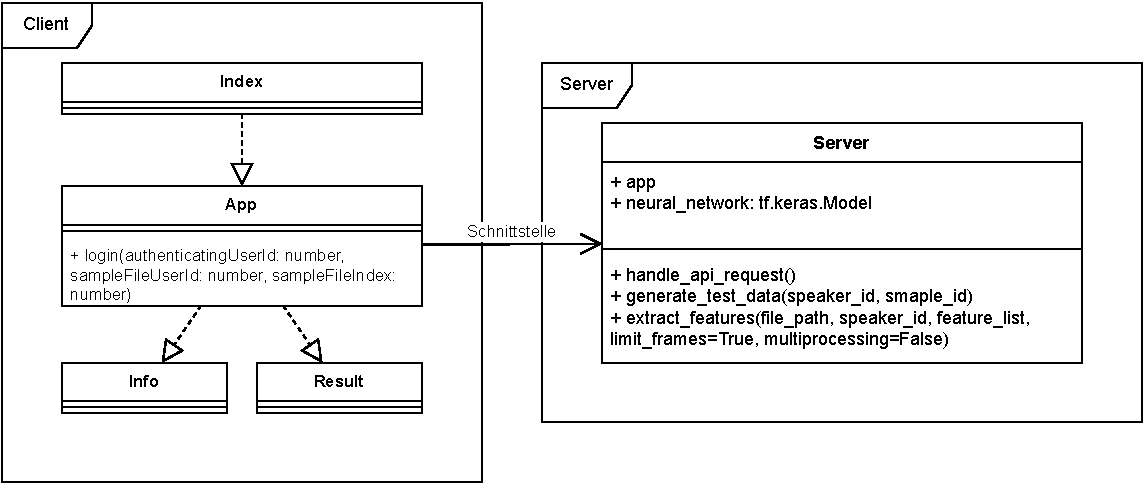
\includegraphics[width=0.9\textwidth, keepaspectratio]{images/Architektur-Demosystem}
    \caption{Architektur Demosystem}
    \label{fig:ArchitectureDemoSystem}
\end{figure}

\subsubsection{Client}
Der Client wird wie bereits erwähnt als Weboberfläche konzipiert.
Dabei stellt er Eingabemöglichkeiten in Form eines Logins bereit, die für das Anstoßen des Authentifizierungsprozesses benötigt werden.
Im Architekturbild geschieht dies über die \textKlasse{App} Komponente.
Über die \textFunktion{login()} Funktion der Komponente wird die Authentifizierungsanfrage an den Server gestellt.

Dabei werden die Daten \textVariable{authenticatingUserId}, \textVariable{sample\-File\-User\-Id} und \textVariable{sample\-File\-Index} über eine Schnittstelle übermittelt.
Da sich das Demosystem auf einen vordefinierten Datensatz beschränkt muss keine Funktion zur Aufnahme neuer Sprechdaten bereitgestellt werden.
Aus diesem Grund werden vordefinierte Audiosequenzen für jeden Sprecher bereitgestellt, die mittels den Variablen \textVariable{sampleFileUserId} und \textVariable{sampleFileIndex} eindeutig identifiziert werden können.

Die Darstellung des Ergebnisses des Authentifizierungsprozesses wird in eine separate Komponente namens \textKlasse{Results} ausgelagert.
Hierbei handelt es sich um eine reine darstellende Komponente.

Für eine verbesserte Nutzerfreundlichkeit wird zusätzlich eine \textKlasse{Info} Komponente eingebunden, welche die grundlegende Bedienung und Vorgehensweise des Demosystems erklärt.

\subsubsection{Server}
Der Server stellt einen Schnittstellenendpunkt bereit, der Authentifizierungsanfragen eines Clients annimmt, verarbeitet und beantwortet.
In Abbildung~\ref{fig:SequenceHandleApiRequest} ist ein exemplarischer Ablauf des gesamten Prozesses modelliert.

\begin{figure}[H]
    \centering
    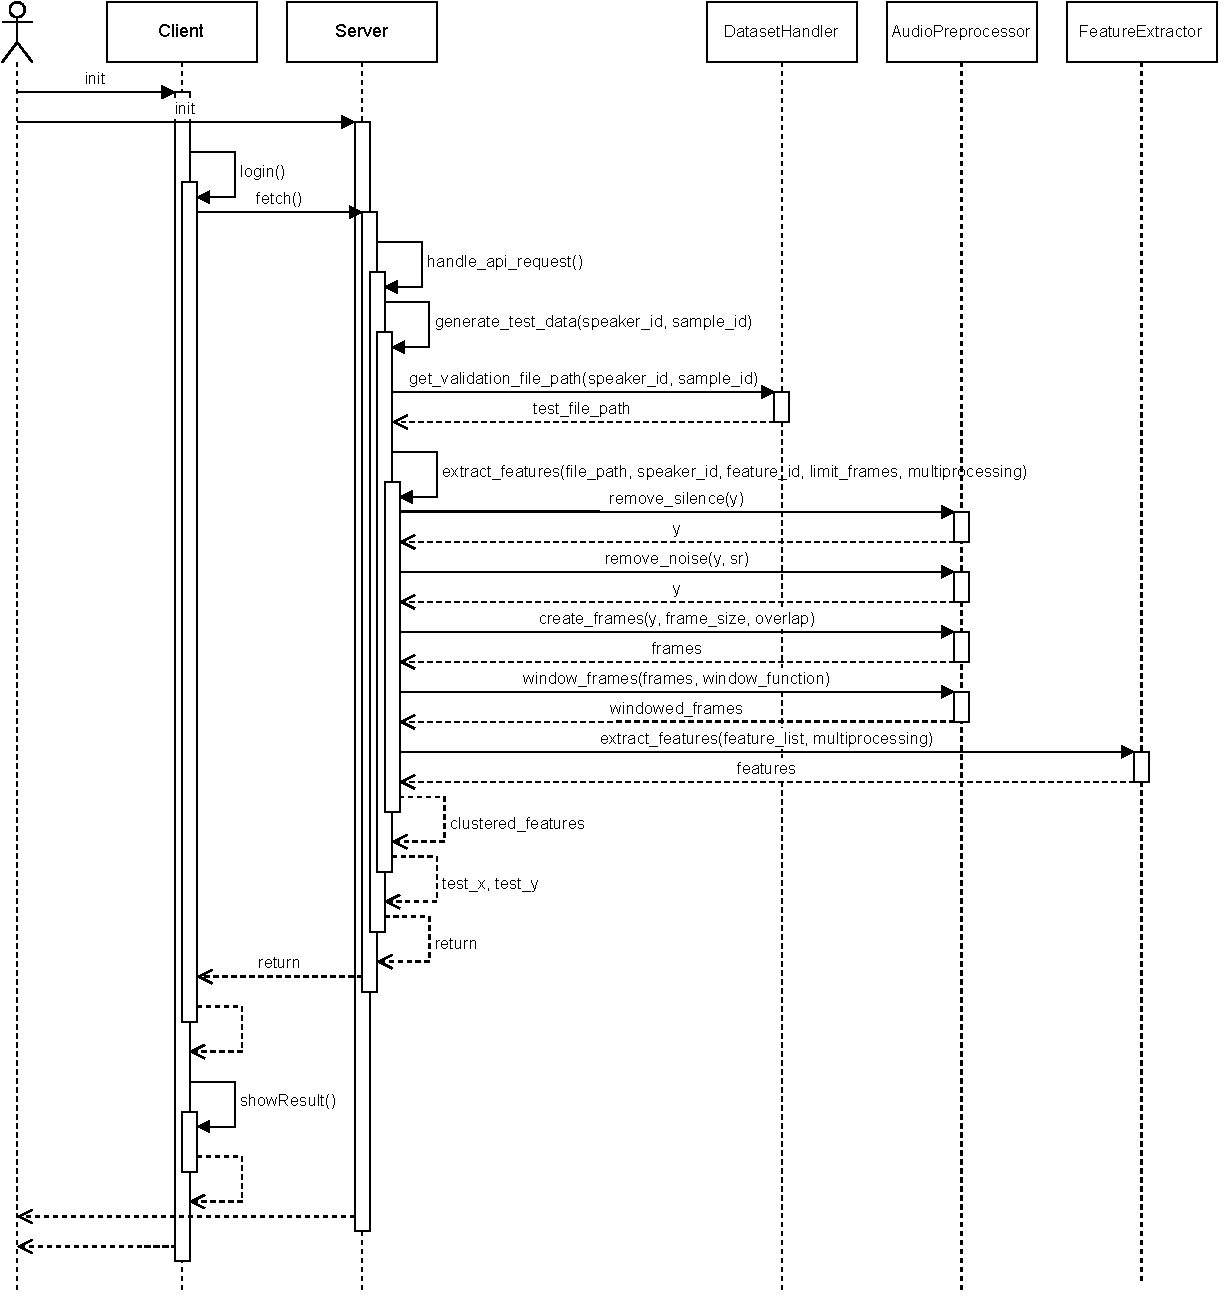
\includegraphics[width=0.9\textwidth, keepaspectratio]{images/SequenzdiagrammClientServer}
    \caption{Sequenzdiagramm login()}
    \label{fig:SequenceHandleApiRequest}
\end{figure}

Eine eingehende Authentifizierungsanfrage wird von der Funktion \textFunktion{handle\_api\_request()} verarbeitet.
Die Klassifizierung der übergebenen Audiodatei verläuft dabei analog zum Versuchssystem, weshalb hier die Komponenten des Versuchssystems (\textKlasse{Dataset\-Handler}, \textKlasse{Audio\-Preprocessor}, \textKlasse{Feature\-Extractor}) innerhalb der Funktionen \textFunktion{generate\_test\_data()} und \textFunktion{extract\_features()} genutzt werden können. % TODO: Evtl. Referenz auf Versuchssystem Konzept

Die Ergebnisse der Authentifizierung werden über die Schnittstelle zurück an den Client gesendet.

\subsubsection{Schnittstellendefinition}
Im Konkreten enthält die Anfrage des Clients die folgenden Informationen:
\begin{itemize}
    \item Zu authentifizierender Sprecher
    \item Index der ausgewählten Sprachdatei
    \item Sprecher der ausgewählten Sprachdatei
\end{itemize}
Die Antwort des Servers beinhaltet die Informationen:
\begin{itemize}
    \item Ermittelte Wahrscheinlichkeit des zu authentifizierenden Sprechers
    \item Authentifizierungsstatus
    \item Ermittelte Wahrscheinlichkeit je Sprecher
\end{itemize}

\textauthor{\vHS}{}{}
  \section{Umsetzung}

Das vorliegende Kapitel befasst sich mit der Umsetzung des Versuchssystems und des Demosystems.
Dazu wird zunächst eine Technologieentscheidung für das Versuchssystem getroffen, auf Basis dieser, wird auch eine Entscheidung für das Demosystem getroffen.
In einem weiteren Schritt wird die systematische Umsetzung der beiden Systeme dargestellt.

\subsection{Technologieentscheidung}

\subsubsection{Versuchssystem}\label{sec:TechnologieVersuchssystem}

Aus der Konzeption in Kapitel~\ref{sec:Konzeption} gehen verschiedene Anforderungen an die Technologie hervor.
Durch die Verwendung von neuronalen Netzen werden die verfügbaren Technologien bzw. Programmiersprachen bereits eingeschränkt.
Um weitere Technologieenscheidungen zu treffen, muss zunächst eine Programmiersprache ausgewählt werden.
Da in einer Umfrage unter Machine-Learning-Entwicklern und Data Scientists 57\% Python als Programmiersprache nutzen und 33\% diese sogar priorisieren, wird für dieses Projekt Python als Programmiersprache festgelegt \autocite[vgl. ][S. 16]{vision_mobile_state_2017}.
In einer allgemeinen Umfrage zu verwendeten Programmiersprachen liegt Python mit 49,2\% auf Platz drei \autocite[vgl.][]{yepis_2023_2023}.
Das bedeutet, dass knapp die Hälfte der befragten Entwickler unter anderem Python verwenden, somit ist eine ausreichende Verbreitung gewährleistet.
Die Verbreitung ist vor allem deshalb ein wichtiger Aspekt, da es durch eine hohe Verbreitung ein großes Eco-System mit vielen quelloffenen Ressourcen und bereits durchgeführten Projekten gibt.

Um Machine-Learning mit Python zu betreiben, gibt es mehrere Bibliotheken zur Auswahl.
Die 3 bekanntesten Open-Source-Bibliotheken sind dabei \gqq{TensorFlow}, \gqq{PyTorch} und \gqq{SciKit-Lern} \autocite[vgl.][]{msv_tensorflow_2020}.

Diese Bibliotheken sind sich relativ ähnlich.
Vorteile einer Bibliothek bringen automatisch auch Nachteile, die sich somit gegenseitig aufheben.

Für diese Studienarbeit wird TensorFlow genutzt, da es laut der \gqq{Stack Overflow Developer Survey 2022} eine größere Nutzerbasis hat \autocite[vgl.][]{stack_overflow_stack_2022}.
Zudem spricht für diese Entscheidung auch die Tatsache, dass die Entwickler dieser Studienarbeit bereits Vorkenntnisse in TensorFlow haben.

Zusätzlich wird das Modul \gqq{Keras} verwendet, welches eine entwicklerfreundliche High-Level-Schnittstelle für TensorFlow ist und somit eine einfachere Entwicklung ermöglicht \autocite[vgl.][]{noauthor_keras_2023}.

\subsubsection{Demosystem}
Für die Technologieentscheidung muss zunächst zwischen den zwei Komponenten Client und Server unterscheiden werden.
Da für beide Teile unterschiedliche Anforderungen erfüllt werden müssen, erfolgt die Technologieentscheidung separat.
Außerdem findet eine Festlegung des verwendeten Protokolls für die Schnittstellenkommunikation statt.

\paragraph{Client}
Die grundlegende Anforderung an den Client ist die Umsetzung als Webapplikation.
Daraus leiten sich in erster Linie vier verschiedene Programmiersprachen ab: JavaScript/Type\-Script, Python, PHP und Ruby.

Für eine weitergehende Einschränkung ist der vorausgesetzte Funktionsumfang relevant.
Dieser ist sehr gering, da lediglich Input-Elemente für die Angabe eines zu authentifizierenden Sprechers, sowie zur Auswahl einer zu verwendeten Datei bereitgestellt werden müssen.
Außerdem muss eine Verbindung zu einem Back-End (Server) aufgebaut werden können.

Da diese Anforderungen durch alle vier Kandidaten erfüllt werden, muss die Entscheidung durch andere Kriterien erfolgen.
Hierbei spielen vor allem zwei Aspekte eine Rolle.
Eine Umfrage von Stack Overflow aus dem Jahr 2020 zeigt, dass JavaScript die beliebteste Programmiersprache von professionellen Entwickler ist.
Moderne Frameworks wie ReactJS und Angular haben die klassische Webprogrammierung in PHP über die letzten Jahre abgelöst \autocite[vgl.][]{stack_overflow_stack_2020}.

Da es sich außerdem um ein Demosystem handelt, welches lediglich die Ergebnisse dieser Arbeit präsentieren soll und somit nicht in einem produktiven Umfeld betrieben wird, spielt die Technologieentscheidung nur eine untergeordnete Rolle.
Die Kompetenzen des Entwicklerteams liegen vor allem im Bereich der React Programmierung mit JavaScript beziehungsweise TypeScript.

Zusammenfassend fällt die Technologieentscheidung für die Client-Implementierung somit auf das JavaScript Framework ReactJS in Kombination mit TypeScript.
TypeScript ermöglicht dabei gegenüber JavaScript die Verwendung von Datentypen, wodurch Datentypfehler im Rahmen der Implementierung vermieden werden können.

\paragraph{Schnittstelle}
Im Web-Umfeld spielt das \ac{HTTP} eine besondere Rolle.
Dabei handelt es sich um ein zustandsloses Protokoll zur Übertragung von Daten auf der Anwendungsschicht.
Ein Anwendungsfall ist dabei die Anfrage von Webseiten im Browser über die URL.
Dazu wird eine sogenannte \ac{HTTP}-GET Anfrage an den Zielserver gesendet, welcher anschließend mit der angeforderten Ressource antwortet.

Nach demselben Prinzip kann das HTTP Protokoll ebenfalls dazu verwendet werden, eine Kommunikation zwischen Client und Server zu ermöglichen.
Die zu übergebenden Variablen des Clients an den Server können dabei innerhalb der URL des GET-Requests übertragen werden.
Gleichzeitig können die Ergebnisse des Servers beispielsweise im JSON-Format an den Client zurückgesendet werden.

Da das HTTP Protokoll somit alle benötigten Anforderungen erfüllt, kommt es für die Schnittstellenkommunikation zum Einsatz.

\paragraph{Server}
Für den Authentifizierungsprozess implementiert der Server denselben Ablauf wie das Versuchssystem.
Um eine doppelte Entwicklung zu vermeiden, entsteht somit eine Abhängigkeit zwischen der Technologieentscheidung des Versuchssystems und des Servers.
Aus der Technologieentscheidung des Versuchssystems in Kapitel~\ref{sec:TechnologieVersuchssystem} geht die Programmiersprache Python hervor.
Somit sollte zunächst geprüft werden, ob die Anforderungen des Servers in der Sprache Python umsetzbar sind.

Neben dem Authentifizierungsprozess spielt ausschließlich die Schnittstellenkommunikation zwischen Client und Server eine Rolle für die Technologieentscheidung des Servers.
Da als Kommunikationsprotokoll HTTP eingesetzt wird, muss also eine Bibliothek gefunden werden, die die Verwendung dieses Protokolls in Python ermöglicht.
Hierzu kann Flask verwendet werden.

Bei Flask handelt es sich um ein Web Framework, welches eine Bereitstellung von \ac{API} Endpunkten, die über das \ac{HTTP} Protokoll abrufbar sind, ermöglicht.

Somit können alle Anforderungen an die Serverapplikation mittels der Programmiersprache Python umgesetzt werden.
Dazu können die bereits entwickelten Komponenten für den Authentifizierungsprozess aus dem Versuchssystem übernommen werden.

\subsection{Versuchssystem}\label{sec:UmsetzungVersuchssystem}

\subsubsection{Feature Kombination}

Wie bereits in Kapitel~\ref{sec:FeatureKombination} erwähnt, müssen zuerst die verschiedenen Konfigurationen erzeugt werden.
Hierzu werden die vorher definierten Werte in einer JSON-Datei erfasst und durch ein eigenes Kombinierungs-Skript alle möglichen Konfiguration mit einer ID erzeugt.

Die Konfigurationswerte für die Kombinierung sind im Listing~\ref{lst-configs} dargestellt.

\begin{lstlisting}[language=Python,numbers=none,caption=Konfigurationsmöglichkeiten,label=lst-configs]
Configs = {
    "amount_of_frames": [10000, 15000],
    "size_of_frame": [400, 600],
    "LPC": {
        "order": [13, 20],
        "weight": [0, 1]
    },
    "MFCC": {
        "order": [13, 20],
        "weight": [0, 1]
    },
    "LPCC": {
        "order": [13, 20],
        "weight": [0, 1]
    },
    "delta_MFCC": {
        "order": [13],
        "weight": [0, 1]
    }
}
\end{lstlisting}

Der \codestyle{weight} Parameter gibt lediglich an, ob in dieser Konfiguration dieses Feature verwendet werden soll oder nicht, um verschiedene Kombinationen zu erreichen.
So gibt es auch manche Kombinationen, die beispielsweise nur \ac{MFCC}-Merkmale in der Analyse berücksichtigen.
Hierbei muss beachtet werden, dass durch die Kombination auch Konfigurationen entstehen, in welchen nichts berechnet werden muss.
Diese werden manuell entfernt.
Die anderen Variablen wie \codestyle{order} und dessen Werte wurde bereits in ~\ref{sec:FeatureKombination} erklärt.

\subsubsection{Datensatz}
Für die Evaluierung der Stimmmerkmale wird ein geeigneter Datensatz benötigt.
Hierzu wurde nach einer Internetrecherche auf der Plattform \gqq{Kaggle} ein entsprechender Datensatz gefunden, der die Anforderung aus Kapitel~\ref{sec:KonzeptDatensatz} erfüllt \autocite[vgl.][]{jain_speaker_2019}. 
Der Originaldatensatz enthält Audiodaten zu 50 Sprechern mit mindestens 60 Minuten Aufzeichnung pro Sprecher in mehreren kompressionslosen WAV Dateien.

In einem ersten Schritt müssen die manuell Daten aufbereitet werden.
Der Originaldatensatz lässt sich in zwei Teile teilen, während der erste Teil aus YouTube Videos besteht, sind im zweiten Teil Aufnahmen von englischen Hörbüchern enthalten.
Da die Aufnahmequalität der Hörbücher deutlich besser ist, wurden nur diese Datensätze weiterverwendet.
In einem Folgeschritt werden die einzelnen Dateien der Datensätze zu einer Datei zusammengefügt und genauer betrachtet.
Hierbei konnten längere Pausen und Abweichungen der Datensätze, wie z.B. mehrere Sprecher oder eine andere Sprache identifiziert werden.
Diese Pausen wurden entfernt und die betroffenen Datensätze aus dem Datensatz entfernt.
Dadurch bleiben 25 geeignete Datensätze übrig, aus diesen wurden unter dem Aspekt des Geschlechts 20 Datensätze ausgewählt, sodass neun weibliche und elf männliche Sprecher im finalen Datensatz sind, da nur neun weibliche Datensätze geeignet sind.
Abschließend wurde für jeden Sprecher eine Audiodatei zum Trainieren des neuronalen Netzes mit acht Minuten erstellt und zur Evaluation neun Sequenzen mit jeweils 15 Sekunden.
Das Testmaterial ist nicht im Trainingsmaterial enthalten.

\subsubsection{Vorverarbeitung und Feature Extraktion}\label{section:umsetzung-versuch-vorverarbeitung}

Um eine effektive Verarbeitung eines Audiosignals zu ermöglichen, muss zunächst eine Vorverarbeitung des Signals erfolgen (s. Kapitel~\ref{sec:preprocessing}).
Hierfür wird der Audio-Clip mittels der Bibliothek \gqq{Librosa} geladen.
Anschließend folgt der erste Schritt der Vorverarbeitung, das Entfernen von stillen Passagen.
Dafür wird ein selbst entwickelter Algorithmus verwendet, der erkennt, wenn sich die Amplitude des Audiosignals über einen gewissen Zeitraum unterhalb eines definierten Schwellwerts befindet.

\begin{lstlisting}[language=Python,numbers=none,caption=Remove Silence,label=lst-remove-silence]
for i, amp in enumerate(y):
if abs(amp) < threshold:
    counter_below_threshold += 1
else:
    if counter_below_threshold > pause_length_in_ms:
        for index in range(i-counter_below_threshold+keep_at_start_and_end, i-keep_at_start_and_end):
            indices_to_remove.append(index)
    counter_below_threshold = 0
\end{lstlisting}

Nach dem Entfernen der Pausen wird das Hintergrundrauschen entfernt.
Dafür wird ein externer Algorithmus von Tim Sainburg verwendet.
Dieser basiert auf dem Vorgehen des bekannten Ton-Verarbeitungsprogramm \gqq{Audacity}.
Zusammengefasst transformiert der Algorithmus mithilfe von \ac{FFT} das Audio-Signal zunächst in den Frequenzraum.
Hier werden dann die Störfrequenzen über Schwellwertverfahren lokalisiert und mittels Filter eliminiert.
Anschließend wird das Signal wieder zurücktransformiert \autocite[][]{sainburg_timsainbnoisereduce_2019}.

Die abschließende Unterteilung des Audiosignals in Frames, sowie das Windowing der Frames findet mit Hilfe von \codestyle{numpy}-Operationen in den Funktionen \codestyle{create_frames} und \codestyle{window_frames} statt.
Die passende Fensterfunktion wird dabei ebenfalls durch die \codestyle{numpy}-Bibliothek bereitgestellt.
Bei dem Aufteilen in Frames wird beachtet, dass sich die Frames überlappen, da sonst durch das Windowing zu viele Informationen verloren gehen würden.

Für das Extrahieren der Merkmale aus dem Audiosignal wird ein Ansatz gewählt, der eine einfache Erweiterung des Programms um verschiedene andere Verfahren ermöglicht.
Dazu wird das Designmuster Strategie in abgewandelter Form verwendet, wobei zunächst ein Interface für die Berechnungsverfahren erstellt werden muss.
Dieses definiert die Funktion \codestyle{calculate_features}, welche in den abgeleiteten Klassen implementiert wird.
Für die eigentlichen Berechnungen der Koeffizienten wird wieder die Signal-Verarbeitungs-Bibliothek Librosa verwendet.
Beispielhaft für die Berechnung von \ac{MFCC} sieht man in Listing~\ref{lst-MFCCExtractor}, wie unkompliziert sich die Bibliothek Librosa verwenden lässt.
Allerdings müssen viele Parameter, wie zum Beispiel die Länge des zu verwendenden FFT-Fenster (\codestyle{n_fft}) gefüllt bzw. geändert werden.
Diese Werte ergeben sich aus den von uns ausgewählten Parameter (beschrieben in~\ref{sec:FeatureKombination}) und den Anweisungen in der offiziellen Dokumentation der Librosa-Bibliothek \autocite[vgl. ][]{librosa_development_team_librosa_2023}

\begin{lstlisting}[language=Python,numbers=none,caption=Klasse zur Extraktion von MFCC-Merkmalen,label=lst-MFCCExtractor]
class MFCCExtractor(ExtractorInterface):

@staticmethod
def calculate_mfcc(frame, sr, order):
    mfcc = librosa.feature.mfcc(y=frame, sr=sr, n_mfcc=order, n_fft=1024, hop_length=512)
    mfcc_of_frame = np.mean(mfcc.T, axis=0)
    return mfcc_of_frame

def calculate_features(self, frames, sr, order, multiprocessing=False):
    if multiprocessing:
        with Pool(8) as p: # run function on 8 cores
            mfccs = p.starmap(self.calculate_mfcc, [(frame, sr, order) for frame in frames])
        return mfccs
    else:
        mfccs = []
        for frame in frames:
            mfccs.append(self.calculate_mfcc(frame, sr, order))
        return mfccs
\end{lstlisting}

Da für die Versuchsreihe sehr viele zeitaufwändige Berechnungen laufen müssen, ist das Extrahieren der Merkmale mit Multiprocessing implementiert.
Hierfür wird die Python-interne Bibliothek \gqq{mutliprocessing} genutzt, um die Berechnung auf mehrere Kerne zu verteilen.

% librosa load 
% remove silence 
% noice_reduce#

% berechnung der Merkmale für Trainings- und Testdaten --> benötigt für Traditionellen Authentifizierungsprozess

\subsubsection{Klassifikation und Evaluierung}
In dem Kapitel~\ref{sec:KonzeptKlassifikation} wurden neuronale Netze als Klassifikationsmodell gewählt, um die zuvor berechneten Merkmale zu evaluieren.
Hierbei werden zuerst neuronale Netze mit den berechneten Trainingsdaten trainiert.
Die Netze bestehen aus drei Hidden-Layer mit jeweils 128, 64 und 32 Neuronen.
Dieser absteigende Aufbau stellt sich bei Versuchen als geeignete Lösung heraus.

Wie bereits im Konzept dargestellt müssen mehrere neuronale Netze trainiert werden, in diesem Fall werden für jede Konfiguration drei neuronale Netze erstellt.

\begin{lstlisting}[language=Python,numbers=none,caption=Erstellen und Trainieren eines neuronalen Netzes,label=lst-nn]
# create model
tf.keras.backend.clear_session()
model = tf.keras.models.Sequential([
    tf.keras.layers.Flatten(input_shape=[input_layer_neurons]),
    *hidden_layer, # 128, 64, 32
    tf.keras.layers.Dense(output_layer_neurons, activation=tf.nn.softmax),
])
model.compile(optimizer=tf.optimizers.Adam(), loss='sparse_categorical_crossentropy', metrics=['accuracy'])

# train model
model.fit(X, y, epochs=epochs)
\end{lstlisting}

Nach dem Training erfolgt die Evaluation der neuronalen Netze, hierzu wird der tatsächliche Authentifizierungsprozess nachgebildet.
Die berechneten Testdaten werden auf die neuronalen Netze angewandt, das neuronale Netz klassifiziert also die Daten, indem es die Features jedes Frames einem der 20 Sprecher zuordnet.
Diese Klassifizierung wird durch die Tensorflow-Methode \codestyle{model.predict()} realisiert, wie das Listing~\ref{lst-model-predict} zeigt.

\begin{lstlisting}[language=Python,numbers=none,caption=Evaluation mit model.predict und Normalisierung des Ergebnisses,label=lst-model-predict]
prediction = self.neural_network.predict(np.asarray(self.test_data_x[i])) # generate prediction for the sample
correspondence = {} # mapping: speaker to result
for id in range(20): # for each speaker
    correspondence[f"{id}"] = np.count_nonzero(np.argmax(prediction, axis=1) == id) / len(prediction) # normalization
\end{lstlisting}

Die Anzahl der Frames ist dabei von der Frame-Länge der jeweiligen Konfiguration abhängig, weshalb die Zuordnungsverteilungen normiert, also von einer absoluten in eine relative Zuordnung umgerechnet, werden müssen.

Da für jeden Sprecher fünf Testdateien verwendet werden (die Schleife hierfür wird übersichtlichkeitshalber nicht in den Listings gezeigt), entstehen pro neuronalem Netz 100 Zuordnungsverteilungen.
Durch die Berechnung von drei neuronalen Netzen pro Konfiguration ergibt dies 300 Zuordnungsverteilungen pro Konfiguration.

Nach Abschluss der Klassifikation aller Features können diese Datensätze ausgewertet werden und somit ein Rückschluss auf die beste Merkmalskombination getroffen werden.
Die Durchführung und Evaluation des Versuchs sind in Kapitel~\ref{sec:Evaluation} dargestellt.

\subsection{Demosystem}
Die Umsetzung von Client und Server ist im Folgenden beschrieben.
Dabei werden lediglich die wichtigsten Aspekte benannt.
Da der Authentifizierungsablauf bereits im vorangehenden Kapitel erläutert wurde, wird in der Umsetzung des Servers nicht mehr darauf eingegangen.

\subsubsection{Client}
Durch die Verwendung von ReactJS wird die Ordnerstruktur durch das Framework vorgeschrieben.
Diese ist in Abbildung~\ref{fig:OrdnerstrukturClient} dargestellt.
\begin{figure}[H]
    \dirtree{%
      .1 /.
      .2 public.
      .3 audio\_dataset.
      .4 Speaker0000.
      .4 Speaker0001.
      .4 ....
      .3 ....
      .2 src.
      .3 app.
      .4 App.tsx.
      .4 App.css.
      .3 shared.
      .4 components.
      .5 Info.
      .6 Info.tsx.
      .6 Info.css.
      .5 Result.
      .6 Result.tsx.
      .6 Result.css.
      .3 index.tsx.
      .3 index.css.
      .3 ....
      .2 ....
    }
    \caption{Ordnerstruktur Demosystem Client}
    \label{fig:OrdnerstrukturClient}
\end{figure}
Die Projektspezifischen Dateien befinden sich dabei in dem Unterordner \textOrdner{public}, sowie \textOrdner{src}.
Über den \textOrdner{public}-Ordner können Ressourcen wie Bilder oder sonstige Objekte die durch die Website angezeigt werden zur Verfügung gestellt werden.
Sie können dadurch ebenfalls direkt über die URL im Browser abgerufen werden.

Die aufrufbaren Webseiten befinden sich im \textOrdner{src}-Ordner.
Der \ac{HTML}-Code ist in ReactJS in den \textOrdner{*.tsx} Dateien enthalten und erlaubt somit die direkte Einbindung von JavaScript Variablen in die \ac{HTML} Komponenten.
Da es sich bei der Client-Applikation um eine Single Page Application handelt, stellt die \textOrdner{index.tsx} Datei den einzigen Einstiegspunkt der Applikation dar.
Darin wird die Komponente \textKlasse{App} aus der Datei \textOrdner{App.tsx} eingebunden.

Zusätzlich können einzelne Komponenten in separate Dateien ausgelagert werden um auf der einen Seite eine bessere Codeübersicht zu erzeugen und auf der anderen Seite einzelne Visualisierungen an verschiedenen Stellen zu implementieren.
Diese Komponenten werden in dem Unterordner \textOrdner{src/shared/components} abgelegt.

Die Benutzeroberfläche der \textKlasse{App} Komponente zeigt eine Login-Abfrage (siehe Abbildung~\ref{fig:AppLogin}).
\begin{figure}[H]
    \begin{subfigure}[c]{0.49\textwidth}
        \centering
        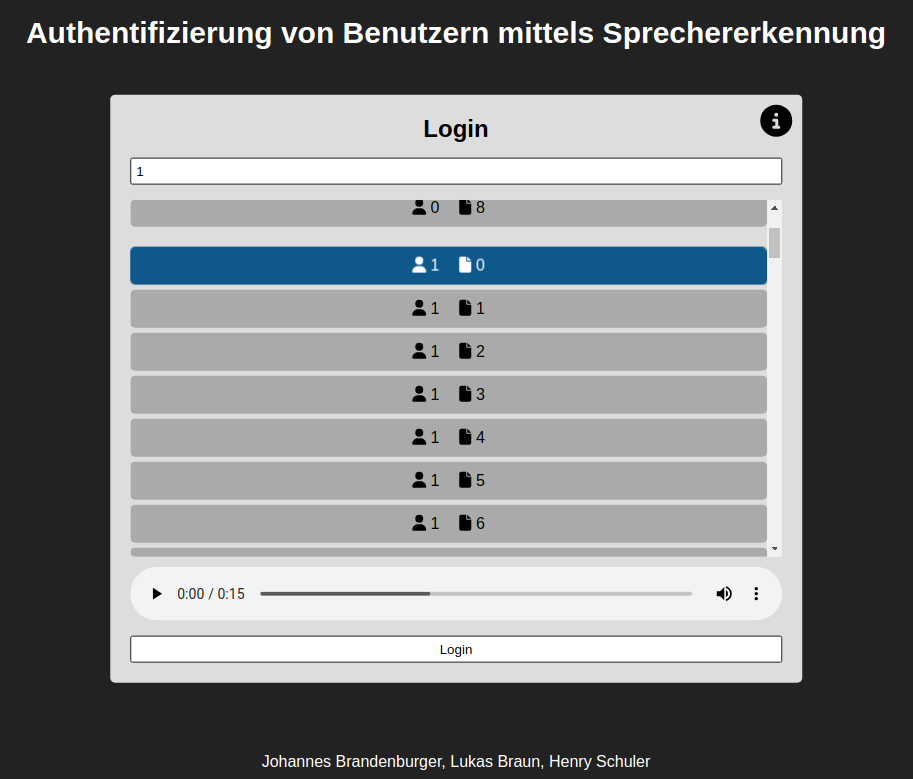
\includegraphics[width=0.9\textwidth, keepaspectratio]{images/UI.png}
        \subcaption{App/Login}
        \label{fig:AppLogin}
    \end{subfigure}
    \begin{subfigure}[c]{0.49\textwidth}
        \centering
        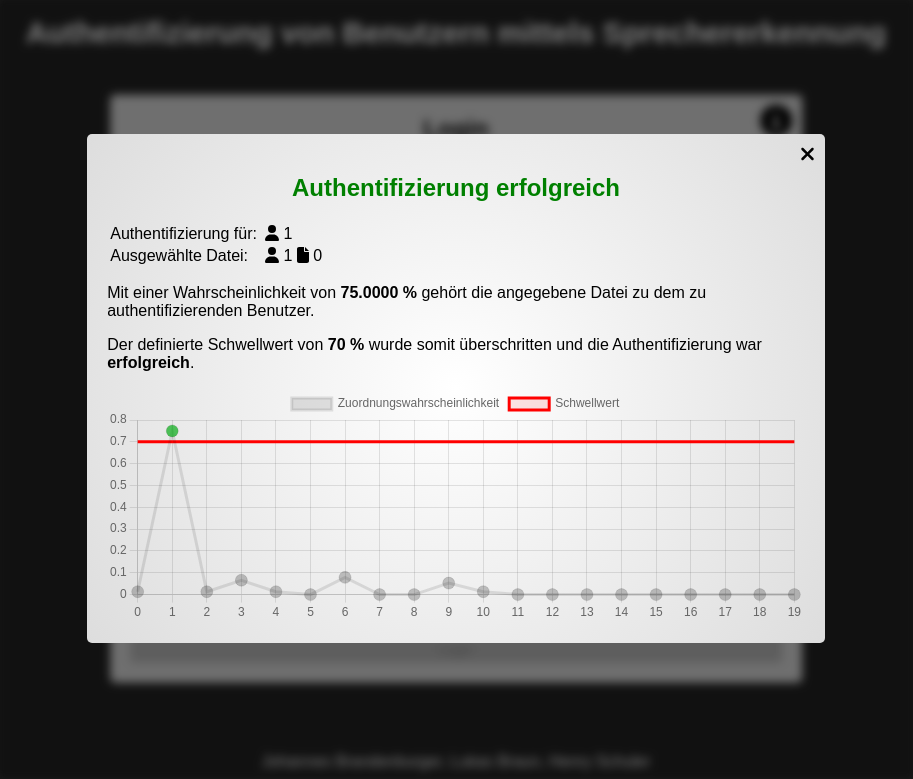
\includegraphics[width=0.9\textwidth, keepaspectratio]{images/UIResult.png}
        \caption{Result}
        \label{fig:Result}
    \end{subfigure}
    \caption{Weboberfläche}
\end{figure}
Diese unterteilt sich in zwei Abschnitte.
Zunächst kann über ein Eingabefeld die ID des zu authentifizierenden Nutzers angegeben werden.
Die Eingabe ist dabei auf die Zahlen 0-19 begrenzt.
Die Eingabe anderer Zeichen führt dazu, dass der Inhalt des Eingabefelds gelöscht wird.
Anschließend kann eine zu verwendende Audiodatei aus einer Liste ausgewählt werden.
Für die Erzeugung der Liste in der Benutzeroberfläche, wird die JSX-Funktion \textFunktion{map()} verwendet um Schaltflächen für jeweils neun Dateien pro Sprecher zu generieren (vgl. Listing~\ref{lst:AudiodateiAuswahl}, Z.~\ref{line:MapOneAppTsx},\ref{line:MapTwoAppTsx}).
Über einen \textFunktion{onClick()} Event-Listener (Z.~\ref{line:OnClickAppTsx}) wird dabei der jeweilige Index des selektierten Elements gespeichert.
\lstset{escapeinside={//(*@}{@*)}}
\begin{lstlisting}[language=HTML,caption=Auswahl der Audiodatei - App.tsx,label=lst:AudiodateiAuswahl]
<div className="fileList">
    {
        // create an array with all numbers from 0 to 20
        Array.from(Array(20).keys()).map((id) => { //(*@\label{line:MapOneAppTsx}@*)
            return Array.from(Array(9).keys()).map((fileIndex) => { //(*@\label{line:MapTwoAppTsx}@*)
                return (
                    <div 
                        key={"speaker" + id + "file" + fileIndex}
                        className={"fileItem " + (sampleFileUserId === id && sampleFileIndex === fileIndex ? "selected" : "")}
                        onClick={() => { //(*@\label{line:OnClickAppTsx}@*)
                            setSampleFileUserId(id);
                            setSampleFileIndex(fileIndex);
                        }}
                    >
                        <span>
                            <FontAwesomeIcon icon={faUser} />
                            &nbsp;{id}
                        </span>
                        <span>
                            <FontAwesomeIcon icon={faFile} />
                            &nbsp;{fileIndex}
                        </span>
                    </div>
                )
            })
        })
    }
</div>
\end{lstlisting}

Um die Benutzerfreundlichkeit zu verbessern besteht dabei zusätzlich die Möglichkeit, die ausgewählte Datei im Browser abzuspielen.
Dafür wird (wie in Listing~\ref{lst:AudioAppTsx} dargestellt) der \ac{HTML} \textFunktion{<audio>} Tag verwendet.
Die dafür benötigten Ressourcen (WAV-Dateien) werden im Ordner \textOrdner{public/audio\_dataset} zur Verfügung gestellt.
\begin{lstlisting}[language=HTML,caption=Audio Tag - App.tsx,label=lst:AudioAppTsx]
<audio controls ref={audioRef}>
    <source src={`./audio_dataset/Speaker${String(sampleFileUserId).padStart(4, '0')}/Validation_Speaker${String(sampleFileUserId).padStart(2, '0')}_${String(sampleFileIndex).padStart(4, '0')}.wav`} type="audio/wav" />
    Audio files are not supported by your browser.
</audio>
\end{lstlisting}

Über den Login-Knopf wird die Authentifizierungsanfrage an den Server gesendet.
Der Knopf kann dabei erst durch den Benutzer gedrückt werden, wenn sowohl in dem Eingabefeld eine valide Zahl steht, als auch eine Authentifizierungsdatei ausgewählt ist.

Für die Anfrage an den Server wird die \textFunktion{fetch()} Funktion von JavaScript verwendet (Z.~\ref{line:FetchAppTsx}).
Die zu übergebenden Parameter werden als URL-Parameter angegeben.
Ist der Server über die angegebene IP-Adresse und Port nicht erreichbar, so wird dies dem Benutzer mittels eines \textFunktion{alert()} mitgeteillt (Z.~\ref{line:AlertAppTsx}).
\begin{lstlisting}[language=JavaScript,caption=login() App.tsx,label=lst:LoginAppTsx]
async function login(authenticatingUserId: number, sampleFileUserId: number, sampleFileIndex: number) {
    try {
        const response = await fetch(`http://${configData.SERVER_URL}:${configData.SERVER_PORT}/?speaker_id=${sampleFileUserId}&sample_id=${sampleFileIndex}&selected_speaker_id=${authenticatingUserId}`); //(*@\label{line:FetchAppTsx}@*)
    
        console.log(response)
        if (!response.ok) {
            return { 
                absolute_accuracy_of_selected_speaker: 0,
                is_authenticated: false,
                absolute_accuracy_of_all_speakers: []
            };
        }
    
        const json = await response.json();
        
        return json;
    } catch (e) {
        console.error(e);
        alert(`Es konnte keine Verbindung zum Server (${configData.SERVER_URL}:${configData.SERVER_PORT}) hergestellt werden!`) //(*@\label{line:AlertAppTsx}@*)
        return {
            absolute_accuracy_of_selected_speaker: 0,
            is_authenticated: false,
            absolute_accuracy_of_all_speakers: []
        }
    }
}
\end{lstlisting}

Die Darstellung des Ergebnisses mittels der \textKlasse{Result} Komponente ist in Abbildung~\ref{fig:Result} dargestellt.
Dem Benutzer werden sowohl seine Authentifizierungsangaben, als auch das Ergebnis der Authentifizierung in Textform angezeigt.
Die Klassifikation als \gqq{erfolgreich} oder \gqq{fehlgeschlagen} kann sowohl dem Text als auch der Farbe der Überschrift (grün oder rot) entnommen werden.

Zusätzlich erhält der Benutzer einen grafischen Einblick in die Wahrscheinlichkeitsverteilung der Zuordnung der ausgewählten Sprecherdatei zu den verschiedenen Sprechern.
Das Diagramm wird mit Hilfe der Bibliotheken chart.js und react-chartjs-2 eingebunden.

\subsubsection{Server} \label{sec:UmsetzungServer}
Wie in der Technologieentscheidung bereits erwähnt, wird der Server mithilfe der Bibliothek Flask implementiert.
Listing~\ref{lst:serverPy} zeigt dabei die wesentlichen Codeabschnitte für die Umsetzung des Servers als Flask Applikation.
\begin{lstlisting}[language=Python,caption=Ausschnitt server.py,label=lst:serverPy]
app = Flask(__name__) //(*@\label{line:FlaskAppServerPy}@*)
CORS(app)

@app.route("/", methods=["GET", "POST"])
def handle_api_request():
    ...

if __name__ == '__main__':
    app.run(debug=False, host='127.0.0.1', port=5500) //(*@\label{line:AppRunServerPy}@*)
\end{lstlisting}
Zunächst muss eine neue Flask \textVariable{app} erstellt werden (Z.~\ref{line:FlaskAppServerPy}).
Mittels \textFunktion{CORS(app)} wird dabei sichergestellt, dass eine Verbindung zwischen Client und Server trotz unterschiedlichem Ursprung möglich ist.

Die Authentifizierungsfunktion wird über die Wrapper-Funktion \textFunktion{handle\_api\_request()} und dem Decorator \textFunktion{@app.route()} als \ac{API} Endpoint verfügbar gemacht.
Die Abarbeitung der Anfragen unterteilt sich in die in Abbildung~\ref{fig:AblaufdiagrammServerHandleApiRequest} dargestellten fünf Schritte.
\begin{figure}[H]
    \centering
    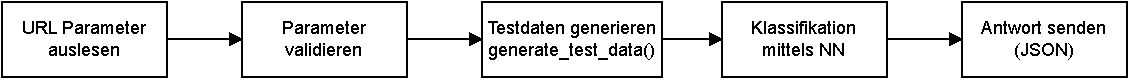
\includegraphics[width=0.9\textwidth, keepaspectratio]{images/AblaufdiagrammServerHandleApiRequest.pdf}
    \caption{Ablauf handle\_api\_request()}
    \label{fig:AblaufdiagrammServerHandleApiRequest}
\end{figure}
Dafür werden zunächst die übergebenen Parameter aus der URL ausgelesen.
Anschließend wird überprüft ob es sich bei den Werten um numerische Werte handelt, die im vorgegebenen Definitionsbereich liegen (vgl. Listing~\ref{lst:ParameterValidationServerPy}).
\begin{lstlisting}[language=Python,caption=Parametervalidierung handle\_api\_request() - server.py,label=lst:ParameterValidationServerPy]
if not (
    speaker_id.isnumeric() and 
    sample_id.isnumeric() and 
    selected_speaker_id.isnumeric() and
    0 <= int(speaker_id) <= 19 and
    0 <= int(sample_id) <= 8 and
    0 <= int(selected_speaker_id) <= 19
):
    return parameter_error_message
\end{lstlisting}
% TODO: evtl. Ref auf genaues Kapitel aktualisieren
Da die Generierung der Testdaten analog zu Kapitel~\ref{sec:UmsetzungVersuchssystem} verläuft, wird darauf nicht weiter eingegangen.
Mit den generierten Daten wird anschließend die Klassifikation durch das \ac{NN} durchgeführt und die Ergebnisse aufbereitet und im JSON-Format an den Client zurück gesendet.

Das neuronale Netz, welches vom Server für die Authentifizierung von Benutzern verwendet wird, ergibt sich aus der Evaluation des Versuchssystems im nachfolgenden Kapitel~\ref{sec:Evaluation}.
Hierzu wird mit der ermittelten Konfiguration ein neues neuronales Netz unter Verwendung von einer erhöhten Anzahl an Epochen generiert, um die Genauigkeit des Systems noch einmal zu verbessern.
Vorgreifend muss hierbei erwähnt werden, dass das System durch die Erhöhung der Epochen insofern verbessert werden konnte, dass die Grenze für die Anzahl an Frames die dem zu authentifizierenden Nutzer zugeordnet werden müssen, von 65 \% auf 70 \% erhöht werden kann.
Deshalb zeigt die Abbildung~\ref{fig:Result} in der Wahrscheinlichkeitsverteilung einen Threshold von 70 \%.

Über die Anweisung \textFunktion{app.run()} unter Angabe der IP-Adresse und des Ports, kann der Server gestartet werden (Listing~\ref{lst:serverPy}, Z.~\ref{line:AppRunServerPy}).
  \section{Evaluation} \label{sec:Evaluation}
% TODO durchführung ??
In dem vorliegenden Kapitel wird die Evaluierung der Ergebnisse des Versuchssystems durchgeführt, hierzu werden die Ergebnisse aufbereitet und anhand mehrerer Metriken verglichen.

Für die Auswertung der Zuordnungsverteilungen aller Konfigurationen des Versuchssystems werden die Ergebnisse zunächst grafisch dargestellt.
Dabei werden in allen Grafiken die Ergebnisse der drei neuronalen Netze pro Konfiguration miteinander Verrechnet.
Es werden vier verschiedene Aspekte betrachtet (vgl. Abbildung~\ref{fig:AuswertungVersuchssystem}).
\begin{figure}[H]
    \centering
    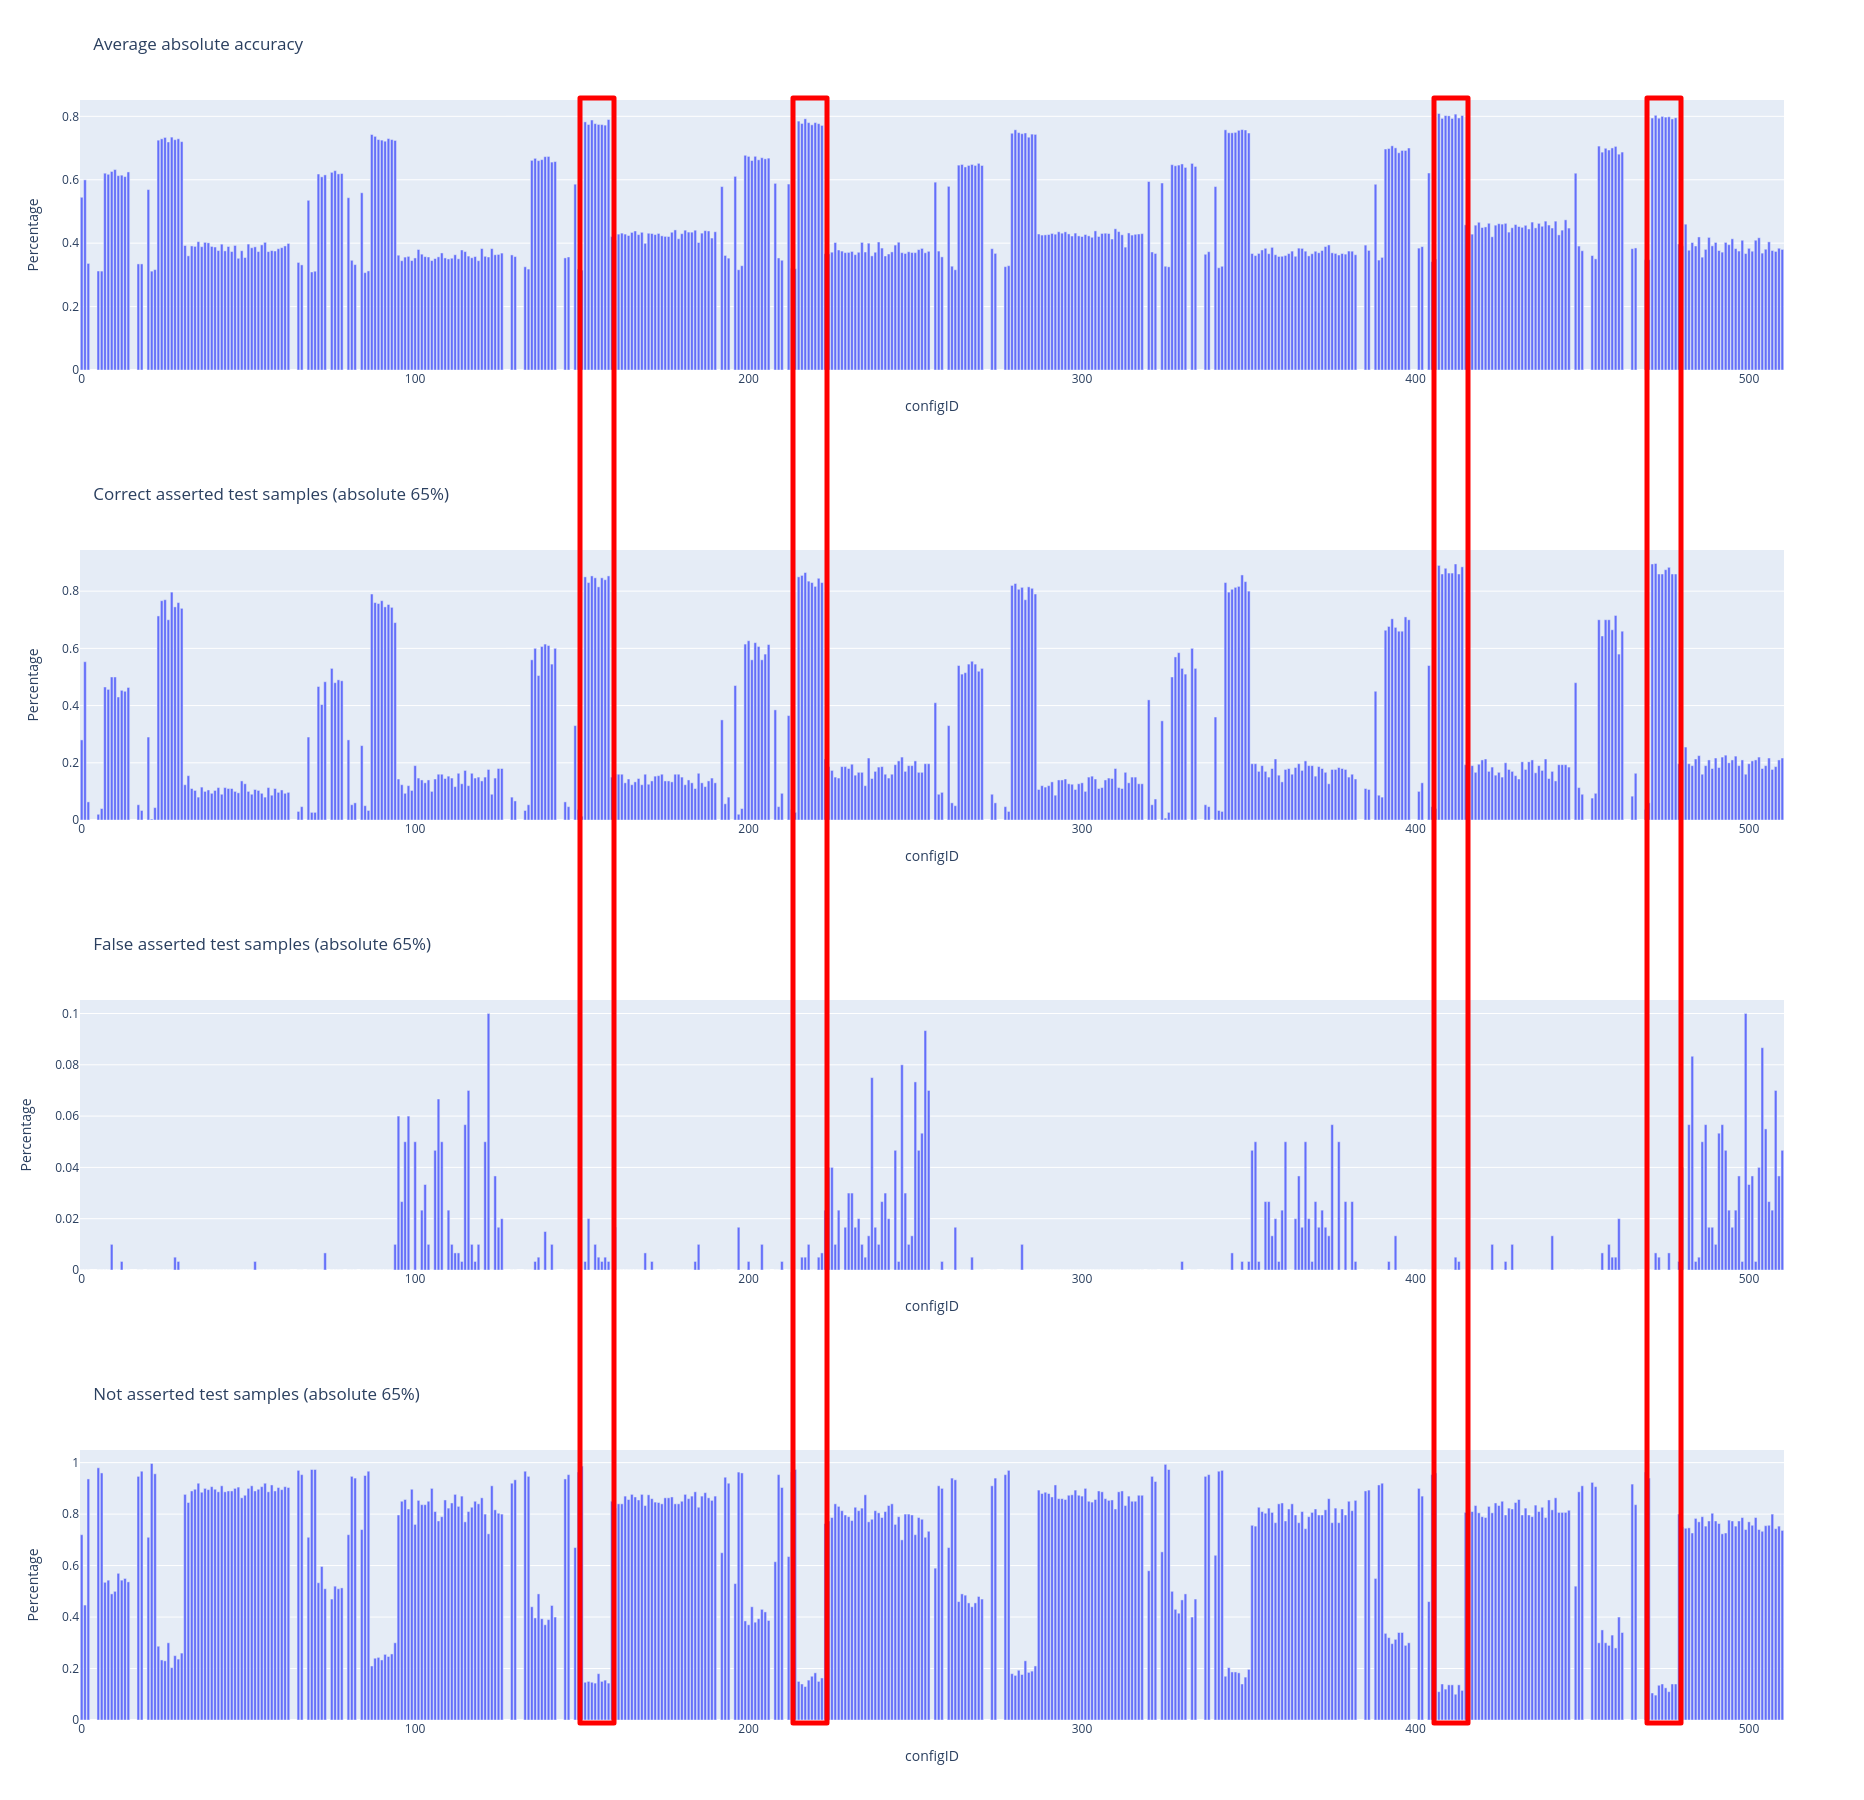
\includegraphics[width=1\textwidth, keepaspectratio]{images/Auswertung.png}
    \caption{Auswertung Versuchssystem}
    \label{fig:AuswertungVersuchssystem}
\end{figure}

Für die durchschnittliche absolute Genauigkeit (erstes Diagramm) werden die Wahrscheinlichkeiten für den zu identifizierenden Benutzer pro Testdatei aufsummiert und der Durchschnitt gebildet.
Eine Genauigkeit von 80 \% entspricht damit der Aussage, dass das neuronale Netz in Kombination mit der jeweiligen Konfiguration dem zu authentifizierenden Benutzer im Durchschnitt 80 \% der Frames der Testdatei zuordnet.

% TODO: Eingehen auf Closed-Set sobald die Entscheidung im Konzept beschrieben ist (Threshold)
Bereits in dieser Grafik zeigt sich die Bildung von Clustern.
Die besten Konfigurationen erreichen eine Genauigkeit von über 65 \%, weshalb dieser Wert für die folgenden drei Auswertungen verwendet wird.
Hier werden die Testdateien mittels dieses Wertes in die drei Kategorien korrekt zugeteilt, falsch zugeteilt und nicht zugeteilt eingeordnet.

Eine Testdatei gilt als korrekt zugeteilt, wenn dem zu authentifizierenden Benutzer mindestens 65 \% der Frames zugeordnet werden.
Analog gilt die Testdatei als nicht korrekt zugeteilt, wenn einem anderen Benutzer mindestens 65 \% der Frames zugeordnet werden.
Erreicht kein Nutzer mindestens 65 \%, so wird die Testdatei als nicht zugeteilt eingestuft.

Für die Bewertung der Konfigurationen gibt es grundsätzlich zwei unterschiedliche Ansätze.
Zunächst kann eine Konfiguration anhand der Anzahl an richtig zugewiesenen Samples bewertet werden.
Dabei steht der Fokus besonders darauf, dass möglichst viele Sprecher möglichst zuversichtlich erkannt und damit auch authentifiziert werden.
In dieser Betrachtung wird allerdings die Anzahl an falsch, beziehungsweise nicht zugewiesenen Samples vernachlässigt, was bedeutet, dass es trotz einer hohen Anzahl an richtigen Zuweisungen auch eine verhältnismäßig hohe Anzahl an falschen Zuweisungen geben kann.
Dies bedeutet für das System, dass die Wahrscheinlichkeit erhöht ist, dass sich eine Person als einen anderen Benutzer ausgeben und authentifizieren kann.

Der dazu gegenteilige Ansatz fokussiert sich auf die Anzahl der falsch zugeordneten Samples.
Um das System möglichst sicher zu halten, sollte diese Zahl minimal (im Optimalfall null) sein.
Es wird also sichergestellt, dass sich keine Person als ein anderer Benutzer erfolgreich authentifizieren kann.
Im Gegenzug kann dies jedoch bedeuten, dass die Anzahl an richtig zugewiesenen Samples sinkt, beziehungsweise die Anzahl der nicht zugewiesenen Samples steigt.
Somit ist die Wahrscheinlichkeit erhöht, dass ein Authentifizierungsversuch trotz korrektem Sprecher fehlschlägt und gegebenenfalls öfters wiederholt werden muss.

Für die Bewertung der Ergebnisse zum Einsatz in dem in dieser Arbeit entwickelten Demosystem wird eine Kombination der beiden Ansätze verfolgt.
Priorisiert wird hierbei der erste Ansatz, also die Orientierung an dem Datensatz mit den Meisten richtig zugeordneten Testdateien um eine gute Benutzerfreundlichkeit zu erzielen.
Gleichzeitig wird aber auch darauf geachtet, dass die Anzahl der falsch zugeordneten Samples möglichst gering ist.
Der Anzahl der nicht zugewiesenen Samples wird eine geringe Wichtigkeit zugeschrieben, da durch die Optimierung der zwei anderen Werte automatisch ein akzeptabler Wert gewährleistet ist.
Außerdem sind die Folgen einer hohen Anzahl nicht zugeordneter Sample vergleichsweise gering, da zunächst keine Authentifikation stattfindet und die Authentifikation mit einem neuen Testsample wiederholt werden kann.

Unter Betrachtung der durchschnittlichen absoluten Genauigkeit, sowie der korrekt zugeteilten Testdateien (zweites Diagramm), ergeben sich die vier markierten Cluster als beste Konfigurationen.
Auch in den zwei verbleibenden Kategorien, zeichnen sich diese Konfigurationen vor allem durch eine niedrige Anzahl an nicht zugeordneten Dateien (kleiner 25 \%, viertes Diagramm), sowie falsch zugeordneter Dateien (kleiner 2 \%, drittes Diagramm) aus.

Die Bildung der Cluster ist dabei auf die Art und Weise wie die Konfigurationen erzeugt werden zurückzuführen.
Da hier eine bestimmte Systematik vorliegt, enthalten diese Cluster jeweils ähnliche Feature-Kombinationen, wobei die für die Ergebnisse relevanten Features in jeder Konfiguration des Clusters vorhanden sind.
In den rot markierten Clustern sind dies \ac{MFCC} und \ac{dMFCC} Features.

In einer detaillierteren Analyse im Direktvergleich ergeben sich die in Tabelle~\ref{table:ergebnisOutput} dargestellten Konfigurationen als beste Kombinationen:
\begin{table}[H]
    \centering
    \begin{tabular}{c|c|c|c|c|c}
    ID  & Durchschnittliche absolute Genauigkeit & \ac{LPC} & \ac{MFCC} & \ac{LPCC} & \ac{dMFCC} \\ \hline
    472 &                                 0.8033 &        0 &        20 &         0 &         13 \\ \hline
    474 &                                 0.8015 &        0 &        20 &        13 &         13 \\ \hline
    410 &                                 0.8015 &        0 &        20 &        13 &         13 \\ \hline
    408 &                                 0.7989 &        0 &        20 &         0 &         13 \\ \hline
    414 &                                 0.7986 &        0 &        20 &        13 &         13 \\
    \end{tabular}
    \caption{Auswertung der Konfigurationen}
    \label{table:ergebnisOutput}
\end{table}

Die Evaluation ergibt somit, dass die Konfiguration mit der ID 472 die besten Ergebnisse erzielt.
Dabei werden 1500 Frames bei einer Frame-Größe von 600 Samples generiert.
Daraufhin werden 20 \ac{MFCC} Koeffizienten, sowie 13 \ac{dMFCC} Koeffizienten pro Frame erzeugt, welche durch das neuronale Netz ausgewertet werden.
\ac{LPC} und \ac{LPCC} zeigen in den ausgewählten Konfigurationen keinen signifikanten Mehrwert, weshalb diese nicht verwendet werden.

In einem weiteren Schritt werden basierend auf der Konfiguration 472 weitere Konfigurationen erstellt, um zusätzliche Untersuchungen durchzuführen.
Dabei werden die Parameter Anzahl der Frames, Länge der Frames, sowie Anzahl der \ac{MFCC} Koeffizienten um jeweils einen neuen Wert erweitert, da hier zu erkennen ist, dass eine Erhöhung dieser Werte zu einer Verbesserung des Gesamtergebnisses führt.
Folgend werden die Parameterwerte 20000 Frames, 800 Samples pro Frame und 27 \ac{MFCC} Koeffizienten evaluiert.
Die Parameterverteilung der Konfigurationen sind in Tabelle~\ref{table:additionalKonfigs} dargestellt.
\begin{table}[H]
    \centering
    \begin{tabular}{c|c|c|c|c}
    ID  & Anzahl Frames & Länge Frames & \ac{MFCC} & \ac{dMFCC} \\ \hline
    511 & 20000         & 600          & 20        & 13         \\ \hline
    512 & 15000         & 800          & 20        & 13         \\ \hline
    513 & 15000         & 600          & 27        & 13         \\ \hline
    514 & 20000         & 800          & 20        & 13         \\ \hline
    515 & 20000         & 600          & 27        & 13         \\ \hline
    516 & 15000         & 800          & 27        & 13    
    \end{tabular}
    \caption{Zusätzliche Konfigurationen}
    \label{table:additionalKonfigs}
\end{table}
Die Ergebnisse der Konfigurationen sind in Tabelle~\ref{table:resultAdditionalKonfigs} aufgelistet.
Da wie bereits beschrieben die Anzahl an richtig zugeordneten Samples in der Evaluierung bevorzugt wird, ergibt sich ein neues optimales Modell mit der Konfigurations-ID 516.
Dabei kann ein Anstieg der richtig zugeordneten Samples um 2,6 Prozentpunkte verzeichnet werden.
Diese Verbesserung ist damit auf die Erhöhung der Framelänge, sowie der Anzahl an \ac{MFCC} Koeffizienten zurückzuführen.

\begin{table}[H]
    \centering
    \begin{tabular}{c|c|c|c|c}
        ID            & Durchschn. abs. Genauigkeit & Richtig zug.   & Falsch zug.    & Nicht zug.     \\ \hline
        472           & 0,8033                      & 0,897          & 0,007          & 0,097          \\ \hline \hline
        511           & 0,8123                      & 0,885          & 0,005          & 0,110          \\ \hline
        512           & 0,8159                      & 0,885          & 0,010          & 0,105          \\ \hline
        513           & 0,8083                      & 0,880          & \textbf{0,003} & 0,117          \\ \hline
        514           & \textbf{0,8416}             & 0,900          & 0,007          & 0,093          \\ \hline
        515           & 0,8190                      & 0,877          & 0,007          & 0,117          \\ \hline
        \textbf{516}  & 0,8377                      & \textbf{0,923} & 0,007          & \textbf{0,070} \\ \hline \hline
        Diff 516-472  & +0,0344                     & +0,026         & 0,000          & -0,027
    \end{tabular}
    \caption{Ergebnisse der zusätzlichen Konfigurationen}
    \label{table:resultAdditionalKonfigs}
\end{table}
Dabei muss jedoch mit beachtet werden, dass mit dieser kleinen Verbesserung auch ein zusätzlicher Aufwand kommt.
Auf der einen Seite wird eine längere Audioaufzeichnung zur Authentifizierung benötigt, da die Framelänge um 200 Samples erhöht wird.
Auf der anderen Seite steigt auch der Rechenaufwand, da anstelle von 20 \ac{MFCC} Koeffizienten nun 27 Koeffizienten berechnet werden müssen.

Unter Anbetracht des erhöhten Aufwands wird somit von einer weiterreichenden Analyse abgesehen.
Da die Veränderungen die zu dem verbesserten Ergebnis führen für die einmalige Berechnung des Neuronalen Netzes des Demosystems tragbar sind, wird die für das Demosystem zu verwendende Konfiguration auf die Konfiguration mit der ID \textbf{516} festgelegt.

  \section{Analyse der Sicherheitsrisiken}
In dem vorliegenden Kapitel wird die Analyse der Sicherheitsrisiken von Sprecherauthentifikationssystemen durchgeführt.
Dazu werden mögliche Angriffsszenarien und entsprechende Gegenmaßnahmen vorgestellt.
Dabei wird die Analyse zunächst auf ein allgemeines System bezogen und die erarbeiteten Sicherheitsrisiken dann auf das entwickelte Demosystem bezogen.
Dies ist möglich, da das Demosystem, wessen Entwicklungen in den vorausgegangenen Kapiteln beschrieben wurde, von diesem allgemeinen System abgeleitet ist.

\subsection{Allgemeine Sicherheitsrisiken}
In diesem Abschnitt erfolgt die Analyse der Sicherheitsrisiken für ein allgemeines Sprecherauthentifikationssystem.
Hierbei geht es speziell um Bedrohungen von Sprecherauthentifikationssystemen, allgemeine Risiken von IT-Systemen werden nicht näher beachtet.
Ein solches System wird in Kapitel~\ref{sec:allgemeiner_system_aufbau} dargestellt und erläutert.
Grundsätzlich gibt es drei Arten von Sicherheitsrisiken für Sprecherauthentifizierungssysteme: Voice-Spoofing, Backdoor-Attacken und Eavesdropping.
Im Folgenden sind diese drei Sicherheitsrisiken dargestellt und erläutert.

Voice Spoofing bezieht sich auf die Nachahmung einer bestimmten Stimme oder die Manipulation einer Sprachaufnahme um so jemanden zu täuschen oder Zugriff auf ein System zu erhalten.
Die Nachahmung der Stimme wird auch als Stimmimitation bezeichnet.
Eine Untersuchung der Universität of Birmingham in Alabama zeigt, dass bereits wenige Minuten Audio des Opfers ausreichen, um die Stimme vollständig zu klonen.
Auch die Optionen zur Beschaffung dieser Informationen werden präsentiert.
Der Angreifer kann sich in der Nähe des Opfers aufhalten und Sprachaufnahmen machen, im Internet nach Aufnahmen suchen oder gezielt über Spam-Anrufe die benötigten Daten erhalten \autocite[vgl.][]{katherine_shonesy_uab_2015}.

Die Manipulation einer Sprachaufnahme bedeutet das Anpassen, beziehungsweise das Bearbeiten, des ursprünglichen Audiosignals.
Guangke Chen setzt in seinem Angriffssystem \gqq{FakeBob} auf Pertubation.
Hierbei wird auf ein Audio Quellsignal eine Störung angewandt, die es ermöglicht, dass das attackierte Sprecherauthentifikationssystem einen anderen Benutzer authentifiziert.
Dabei ist es für einen Menschen nicht möglich einen Unterschied zwischen der originalen Aufnahme und der veränderten Aufnahme wahrzunehmen.
\gqq{FakeBob} attackiert hierbei im Black-Box Modus und hat somit lediglich Zugang zu dem Authentifizierungsergebnis und bei zwei von drei Versuchs-Systemen auf die Ergebnisverteilung.
Im Rahmen der Arbeit wird \gqq{FakeBob} auf das Open-Source System \gqq{Kaldi} und auf die kommerziellen Systeme \gqq{Talentedsoft} und \gqq{Microsoft Azure} angewandt.
\gqq{FakeBob} erzielt hierbei eine 100~\% Attack-Succes-Rate bei \gqq{Kaldi} und \gqq{Talentedsoft}, welche sowohl die Verteilung als auch die Entscheidung bereitstellen.
Bei \gqq{Microsoft Azure} steht nur die Entscheidung zur Verfügung.
Hier erreicht \gqq{FakeBob} eine Attack-Success-Rate von 26~\% \autocite[vgl. ][]{chen_who_2020}.

Um biometrischen Spoofing Attacken entgegenzuwirken, gibt es eine sogenannte \ac{PAD}.
\ac{PAD} verwendet verschiedene Techniken und Algorithmen um gefälschte oder vorab aufgezeichnete Sprachaufnahmen zu identifizieren \autocite[vgl. ][]{paravision_introduction_2022}

Backdoor Attacken beschreiben das Vorgehen, bei dem der Hacker gezielt die Trainingsdaten verändert um somit eine Hintertür zu schaffen, über die das System infiltriert werden kann.
Die Untersuchungen von Tongqing Zhai zeigen ein solches Verfahren auf.
Hierzu bearbeitet der Hacker der Trainingsdatensatz, ohne Kenntnis über den eigentlichen Anmeldungsprozess.
In der Arbeit werden unterschiedliche Ansätze zur Veränderung auf zwei Datensätzen durchgeführt.
Hierbei werden Attack Success Rates zwischen mindestens 45~\% und maximal 99,5~\% erreicht \autocite[vgl. ][]{zhai_backdoor_2021}

Um sich vor Backdoor Attacken zu schützen, kann die Integrität des Datensatzes überprüft werden, um so Manipulationen zu identifizieren.
Dies kann beispielsweise durch ein Prüfsummen Verfahren realisiert werden.

Eavesdropping bezeichnet im Allgemeinen das Abhören.
Dies kann im Bezug auf Sprecherauthentifikationssysteme auf unterschiedliche Art und Weise durchgeführt werden.
Grundsätzlich kann der zu authentifizierende Sprecher direkt aufgenommen werden.
Hierzu eignen sich beispielsweise Telefongespräche oder Fake-Interviews.
Diese Aufnahme kann im Anschluss zur Authentifizierung am System verwendet werden.
Alternativ können Angreifer auf online Sprach- bzw. Videoaufnahmen zurückgreifen.

Ein weiterer Ansatz ist das klassische Eavesdropping, hierbei spioniert der Angreifer die Kommunikationsverbindung zwischen Benutzer und System aus und zeichnet diese auf.
Mit dieser Aufzeichnung kann er sich zu späterem Zeitpunkt ebenfalls am System anmelden.

Um oben genannte Eavesdropping Angriffe zu vermeiden, kann vor das Sprecherauthentifikationssystem eine Texterkennung geschaltet werden.
Somit kann durch Vorgabe eines Satzes überprüft werden, ob es sich um eine Aufnahme handelt.
Das klassische Eavesdropping lässt sich durch die Verwendung von verschlüsselten Kommunikationsverbindungen vermeiden.

\subsubsection{Einordnen in die STRIDE-Kategorien}
% TODO Muss Mann das belegen was das ist?
Im Folgenden werden die oben genannten Sicherheitsrisiken in die STRIDE-Kategorien eingeordnet.
Wie bereits oben genannt, werden lediglich spezielle Bedrohungen von Sprecherauthentifikationssystemen behandelt.
STRIDE steht für sechs verschiedene Kategorien zur Bewertung von Sicherheitsrisiken für IT-Systeme (s. Kapitel~\ref{sec:stride}).
% textuell: Paragraph pro Kategorie
\paragraph{Spoofing}
Wie im Namen enthalten fällt unter Spoofing das Voice Spoofing.
Das Risiko besteht darin, dass die Stimme eines autorisierten Sprechers nachgeahmt wird, oder eine manipulierte Sprachaufnahme verwendet wird.

\paragraph{Tampering}
Tampering bedeutet zu Deutsch Manipulation.
Deshalb fällt das Voice Spoofing ebenfalls in die Kategorie Tampering.
Ebenso fällt die Backdoor Attacke in diese Kategorie, da hierbei die Trainingsdaten gezielt manipuliert werden.

\paragraph{Repudiation}
Repudiation bezieht sich auf die Fähigkeit Aktionen innerhalb des Systems zu leugnen, somit kann die Integrität des Systems infrage gestellt werden.
Diese Kategorie findet jedoch auf allgemeine Bedrohungen für Sprecherauthentifikationssystemen keine Anwendung.

\paragraph{Information disclosure}
Information disclosure beschreibt die Offenlegung von vertraulichen Daten.
Dies kann durch Eavesdropping Angriffe auftreten, da ein Angreifer durch Aufzeichnung von Authentifizierungsinformationen Zugang zum System erhalten kann.

\paragraph{Denial of service}
Denial of service bedeutet \gqq{Verweigerung des Dienstes}, bei einer solchen Attacke wird gezielt das System überlastet, um einen Ausfall zu provozieren.
Diese Kategorie findet wie Repudiation keine Anwendung auf allgemeine Bedrohungen für Sprecherauthentifikationssystemen.

\paragraph{Elevation of privilege}
Elevation of privilege beschreibt das Erlangen zusätzlicher Berechtigungen um so Zugang zu weiteren Ressourcen zu erhalten.
In diese Kategorie fällt die Backdoor Attacke, da der Angreifer gezielt die Trainingsdaten verändert, um eine Hintertür zu schaffen, sodass er das System infiltrieren kann.



\subsubsection{DREAD-Analyse}

% Übersichststabelle und dann gleich mit DREAD Bewertung

\subsection{Bezug zum Demosystem}

% textuell


































































  \section{Fazit und kritische Reflexion}
\textauthor{\vHS}{}{}
  \section{Ausblick}


  %%%%%%%%%%%%%%%%%%%%%%% Literaturverzeichnis %%%%%%%%%%%%%%%%%%%%%%%
  \include{pages/literaturverzeichnis}


  %%%%%%%%%%%%%%%%%%%%%%%%%%%%%% Anhang %%%%%%%%%%%%%%%%%%%%%%%%%%%%%%
  \renewcommand{\thetable}{\Alph{section}.\arabic{table}}
  \renewcommand{\thefigure}{\Alph{section}.\arabic{figure}}
  \renewcommand{\thelstlisting}{\Alph{section}.\arabic{lstlisting}}
  \pagenumbering{Alph}

  % \include{pages/anhang}
\end{document}